\documentclass[fleqn,10pt]{wlscirep}

% Packages
\usepackage[super]{nth}
\usepackage{rotating}
\usepackage{makecell}
\usepackage{pifont}
\usepackage{amsfonts}
\usepackage{amsmath}
\usepackage{float}
\usepackage{pgfplotstable}
\usepackage[multiple]{footmisc}

\pgfplotsset{compat=newest}
\usepackage{listings, textcomp}

\lstset{ %
  basicstyle=\ttfamily\footnotesize,  % size of fonts used for the code
  breaklines=true,   % automatic line breaking only at whitespace
  captionpos=b,   % sets the caption-position to bottom
  commentstyle=\color{gray},  % comment style
  keywordstyle=\color{blue},  % keyword style
  stringstyle=\color{red},  % string literal style
  upquote=true  %straight single quotes (requires textcomp)
}

% New Commands
\newcommand{\cmark}{\ding{51}}%
\newcommand{\xmark}{\ding{55}}%
\newcommand{\code}[1]{\texttt{#1}}
\newcommand{\fixme}[1]{\textcolor{red}{{#1}}} 

\title{SciPy 1.0---Fundamental Algorithms for Scientific Computing in Python}

\author[1]{Pauli Virtanen}
\author[2,*]{Ralf Gommers}
\author[3,4]{Tyler Reddy}
\author[5]{Anne Archibald}
\author[6]{Andrew Nelson}
\author[7]{Charles Harris}
\author[8]{CJ Carey}
\author[9]{Denis Laxalde}
\author[10]{Eric Larson}
\author[11]{Eric Moore}
\author[12]{Eric Quintero}
\author[13]{Evgeni Burovski}
\author[14]{Jaime Fernández del Río}
\author[15]{Josef Perktold}
\author[16]{Josh Wilson}
\author[17]{Matthew Brett}
\author[18]{Nikolay Mayorov}
\author[19]{Warren Weckesser}
\author[20]{Matt Haberland}
\author[21]{Scott Sievert}
\author[22]{Yu Feng}
\author[23]{Antonio Horta Ribeiro}
\author[24]{Ian Henriksen}
\author[3,25]{K. Jarrod Millman}
\author[3]{St\'efan J. van der Walt}

\affil[1]{Affiliation, department, city, postcode, country}
\affil[2]{Affiliation, department, city, postcode, country}
\affil[2]{Affiliation, department, city, postcode, country}
\affil[3]{Berkeley Institute for Data Science, University of California, Berkeley, CA, 94720, USA}
\affil[4]{Los Alamos National Laboratory,
	  Theoretical Division 6,
          Los Alamos, NM, 87545, USA}
\affil[5]{Affiliation, department, city, postcode, country}
\affil[6]{Affiliation, department, city, postcode, country}
\affil[7]{Affiliation, department, city, postcode, country}
\affil[8]{Affiliation, department, city, postcode, country}
\affil[9]{Affiliation, department, city, postcode, country}
\affil[10]{Affiliation, department, city, postcode, country}
\affil[11]{Affiliation, department, city, postcode, country}
\affil[12]{Affiliation, department, city, postcode, country}
\affil[13]{Affiliation, department, city, postcode, country}
\affil[14]{Affiliation, department, city, postcode, country}
\affil[15]{Affiliation, department, city, postcode, country}
\affil[16]{Affiliation, department, city, postcode, country}
\affil[17]{Affiliation, department, city, postcode, country}
\affil[18]{Affiliation, department, city, postcode, country}
\affil[19]{Affiliation, department, city, postcode, country}
\affil[20]{BioResource and Agricultural Engineering, California Polytechnic State University, San Luis Obispo, CA, 93407, USA}
\affil[21]{Affiliation, department, city, postcode, country}
\affil[22]{Affiliation, department, city, postcode, country}
\affil[23]{Affiliation, department, city, postcode, country}
\affil[24]{University of Texas at Austin,
           Institute for Computational Engineering and Sciences,
	   Austin, TX, 78712, USA}
\affil[25]{Division of Biostatistics, University of California,
  Berkeley, CA, 94720, USA}

\affil[*]{ralf.gommers@gmail.com}

\keywords{Scientific computing, Python, Mathematics}

% NOTE: some usage stats below are from https://libraries.io/pypi/scipy
% as well as github metrics; normally one doesn't put citations directly
% in abstract though (depends on field / journal)
\begin{abstract}
SciPy is an open source scientific computing library for the Python programming language.
SciPy 1.0 was released in late 2017, about 16 years after the original
version 0.1 release. SciPy
has become a \emph{de facto} standard for leveraging scientific algorithms
in the Python programming language, with more than 600
unique code contributors, millions of downloads per year, 161 dependent
packages, and 28700 dependent repositories. This includes usage of SciPy
in almost half of all machine learning projects on GitHub, and usage by
high profile projects including LIGO gravitational wave analysis and creation
of the first-ever image of a black hole (M87).
The library includes functionality spanning clustering, Fourier transforms,
integration, interpolation, file I/O, linear algebra, image processing,
orthogonal distance regression, minimization algorithms, signal processing,
sparse matrix handling, computational geometry, and statistics. In this
work, we provide an overview of the capabilities and development practices of the
SciPy library and highlight some recent technical developments.
\end{abstract}
\begin{document}

\flushbottom
\maketitle
\thispagestyle{empty}

\section*{Introduction}

%% SciPy is not what you think it is

%% - At risk of failure many times
%% - Funding was *hard* to come by; funding agencies didn't easily give
%%   money.  Some labs, Enthough committed a bit of money.
%% - Java and other enterprize packages were getting support; MATLAB
%%   was huge.  Not many wanted to encourage this ``amateur'' effort.
%% - Graduate students & post-docs doing the heavy lifting; they found
%%   a system they enjoyed using, saw its potential, put energy into it.
%% - Driven by eclectic group of people being passionate about it, not
%%   because they were paid or told to work on it.
%% - And not by EECS people, but by scientists.  Some with fairly little
%%   programming background (David), others in varying stages of academic/research careers.
%% - Over time, the project became more more professional:
%%   - Standardized release formats
%%   - Docstrings
%%   - Testing & CI infrastructure
%%   - APIs
%%   - Issue tracking
%%   - Revision control (CVS -> SVN -> Git)
%%   - Conference
%% - Python wasn't perfectly suited in all ways; packaging, compiling,
%%   indexing (indexing/array protocols and complex numbers added)
%% - Initially, this high quality, stable, widely used project, hinged on
%%   three people doing the ``right'' thing to get it established.
%% - Bus factor for maintenance still very low.

%% The background section captures a selective history where we're trying
%% to identify some of the more important events.  But really, it relies
%% on the collective work of numerous individuals, too many to mention.

SciPy is a library of numerical routines for the Python programming
language that provides fundamental building blocks for modeling and
solving scientific problems. 
SciPy includes algorithms for optimization, integration, interpolation,
eigenvalue problems, algebraic equations, differential equations, and many other
classes of problems; it also provides
specialized data structures, such as sparse arrays
and $k$-dimensional trees. SciPy is built on top of 
NumPy\cite{vanderwalt2011numpy,Oliphant-2015},
which provides array data structures and related fast numerical routines, and
SciPy is itself the foundation upon which higher level scientific libraries,
including scikit-learn\cite{pedregosa2011scikit}
and scikit-image\cite{vanderwalt2014scikit}, are built. 
SciPy is relied upon by scientists, engineers, and others 
around the world. For example, published 
scripts\cite{alex_nitz_2018_1596771, LIGO-open}
used in the analysis of gravitational waves
\cite{PhysRevD.93.122003, abbott2017gw170817} 
import several submodules of SciPy, and the M87 black
hole imaging project directly cites SciPy\cite{2019ApJ875L3E}.

Recently, SciPy released version 1.0, a milestone that traditionally
signals a library's API (Applications Programming Interface) being
mature enough to be be trusted in production pipelines. This version 
numbering convention, however, belies the history of a project that has
become the standard which others follow and has seen extensive
adoption in research and industry.

SciPy's arrival at this point is surprising, and somewhat anomalous.
When started, the library had little funding, and was written mainly
by graduate students---many of them without a computer science education, and often without the
blessing of their advisors.  To even imagine that a small group of
``rogue'' student programmers could upend the already well-established
ecosystem of research software---backed by millions in funding, and
many hundreds of highly qualified engineers\cite{mathworks-globe-97,
esri-revenue,bloom-wolfram}---was preposterous.

Yet, the philosophical motivations behind a fully open toolstack, and
an excited, friendly community with a singular focus, seemed to have
proven auspicious in the long run.  It led not only to the library
described in this paper, but also to an entire ecosystem of related
packages \cite{scipy-ecosystem}, and a variety of social activities centered around
them\cite{social-python}. The packages in the SciPy ecosystem 
share high standards of implementation,
documentation, and testing, and a culture eager to learn and adopt
better practices---both for community management and software
development.

% Despite its success, SciPy still faces challenges:
% a low ``bus factor''---meaning that the entire project depends on a small number of
% active contributors---being perhaps the most serious.

In the background section that follows, we capture a selective history
of some milestones and important events in the growth of SciPy.
Despite what we might highlight here, it is important to understand
that a project like SciPy is only possible because of the
contributions of very many contributors---too many to mention
individually, but each bringing an important piece to the puzzle.

\section*{Background}

Python is an interpreted, high-level, general-purpose computer programming
language, designed by Guido van Rossum in the late 1980s,
with a dynamic type system and an emphasis on readability and rapid prototyping.
The reference and most popular implementation of Python is 
CPython\cite{cpython-refman,cpython-source}, which is written
in the C and Python languages and assumed throughout this paper.
% https://legacy.python.org/search/hypermail/python-1992/0000.html
%
As a general purpose programming language, it had no special support for 
scientific data structures or algorithms, unlike many of the other established
computation platforms of the time. Yet, scientists soon discovered the
language's virtues, such as its ability to wrap C and Fortran
libraries and to then drive those libraries interactively.  Scientists
could thereby gain access to a wide variety of existing computational
libraries without concerning themselves with low-level programming
concepts such as memory management.

In 1995, Jim Hugunin, a graduate student from MIT, wrote the first
message in a new Python Matrix Special Interest Group (Matrix-SIG)
mailing list\cite{Hugunin-first}:
\begin{quote}
There seems to be a fair amount of interest in the Python community
concerning the addition of numeric operations to Python.  My own desire is
to have as large a library of matrix based functions available as possible
(linear algebra, eigenfunctions, signal processing, statistics, etc.).  In
order to ensure that all of these libraries interoperate, there needs to
be agreement on a basic matrix object that can be used to represent arrays
of numbers.
\end{quote}
Over the next several months, conversations on that mailing
list by, among others, Jim Fulton, Jim Hugunin, Paul Dubois, Konrad
Hinsen, and Guido van Rossum, led to the creation of a package called Numeric with an array object
that supported a high number of dimensions.  Jim Hugunin explained the utility
of Python for numerical computation\cite{Hugunin-whitepaper}:
\begin{quote}
I've used almost all of the available numerical languages at one time
or another over the past 8 years. One thing I've noticed is that over
time, the designers of these languages are steadily adding more of the
features that one would expect to find in a general-purpose
programming language.
\end{quote}
This is still a distinguishing feature of Python for science, and one of the
reasons why it has been so successful in the realm of data science: instead of
adding general features to a language designed for numerical and scientific
computing, here scientific features are added to a general purpose language.  
This broadens the scope of problems that can be addressed easily, expands the
sources of data that are readily accessible, and increases the size of the
community that develops code for the platform.

The availability of a standard numerical array data structure in
Python led to a sudden, rapid growth in the number of scientific
packages available for solving common numeric problems.
A number of these packages were written by graduate students and
postdoctoral researchers to solve the very practical research problems
that they faced on a daily basis.  While they had access to and were
familiar with specialized (often commercial) systems, many found
it easier to implement the domain-specific functionality they needed
in a general purpose programming language.  And given Python's innate
ability to function as a systems language, controlling specialized or
custom-built hardware was also possible.

Initial work on numerical computing in Python was driven by graduate
students, but soon larger research labs became increasingly engaged.
For example, Paul Dubois at Lawrence Livermore National Laboratory (LLNL) took over the
maintenance of Numeric and funded the writing of its
manual\cite{Numeric-manual}, and
%in the Program for Climate Model Diagnosis and Intercomparison at
%Lawrence Livermore National Laboratory built their Climate Data
%Analysis Tools (``an open-source set of Python modules and tools for
%accessing, manipulating, and plotting scientific data in general and
%climate data sets in
%particular''\footnote{https://mail.python.org/pipermail/numpy-discussion/2001-May/000645.html})
%on Numeric, the newly established Python array object.  Paul later
%became the maintainer for Numeric, and helped fund the writing of the
%first manual\footnote{https://conference.scipy.org/scipy2010/slides/travis_oliphant_keynote.pdf}
in 1998 the Space Telescope Science Institute (STScI), which was in charge of 
Hubble Space Telescope science operations, decided to replace their
custom scripting language with Python\cite{STScI-slither}.


%Many of the first efforts were driven by graduate
%students and post-doctoral researchers, but soon attracted the
%attention of more senior researchers.
% Paul Dubois, CDAT
% https://mail.python.org/pipermail/numpy-discussion/2001-May/000645.html
% Perry Greenfield, Hubble
% https://conference.scipy.org/scipy2011/slides/greenfield_keynote_astronomy.pdf
%
% Note: plotting was important for them, so they eventually
% funded development on Matplotlib.

% Numeric, even though written by grad students, became critical for
% large scale endeavors



\subsection*{SciPy Begins}

% PhD Mayo Clinic, started faculty position at BYU in 2001
By the late 1990s, discussions appeared on Matrix-SIG
expressing a desire for a complete scientific data analysis environment\cite{Travis-Keynote-2010}.
Travis Oliphant, a PhD student at the Mayo Clinic,
released a number of packages\cite{Travis-some-modules,Travis-enhance} 
that built on top of the Numeric array
package, and provided algorithms for signal processing, special
functions, sparse matrices, quadrature, optimization, Fast Fourier
Transforms, and more.  One of these packages, Multipack, was a set of
extension modules that wrapped Fortran and C libraries such as
ODEPACK, QUADPACK, and MINPACK, to solve and minimize nonlinear
equations, integrate differential equations, and fit splines (the
latter implemented by Pearu Peterson).  Robert Kern, then an
undergraduate student (and currently a SciPy core developer), provided
compilation instructions under Windows.
% 2001 PhD Tallinn Technical University
Around the same time, Pearu Peterson, a PhD student from Estonia,
released F2PY\cite{peterson2009f2py}, a command line tool for binding Python and Fortran
codes, and wrote modules for linear algebra and interpolation.
% Graduated 1999, Duke
Eric Jones, while a graduate student at Duke, wrote a number of
packages to support his dissertation, including a parallel job
scheduler and genetic optimizer.
% Graduated 1998, PhD from Brown, 97–99 postdoc at Harvard Medical
% School; at Harvard ever since
%
% https://mail.python.org/pipermail/scipy-dev/2001-November/000088.html
%
Gary Strangman, a postdoctoral fellow at Harvard Medical School,
published several descriptive and inferential statistical 
routines\cite{Strangman-modules}.

\begin{figure}
\begin{verbatim}
SciPy is an open source package that builds on the strengths of Python and
Numeric providing a wide range of fast scientific and numeric functionality.
SciPy's current module set includes the following:

    Special Functions (Bessel, hanker, Airy, etc.)
    Signal/Image Processing
    2D Plotting capabilities
    Integration
    ODE solvers
    Optimization (simplex, BFGS, Netwon-CG, etc.)
    Genetic Algorithms
    Numeric -> C++ expression compiler
    Parallel programming tools
    Splines and Interpolation
    And other stuff.
\end{verbatim}
\caption{Excerpt from SciPy 0.1 release announcement (typos included).}\label{fig:announce-0.1}
\end{figure}

With a rich programming environment and a numerical array object in
place, the time was ripe for the development of a full scientific
software stack.
In 2001, Eric Jones and Travis Vaught founded Enthought Scientific
Computing Solutions (now Enthought, Inc.) in Austin, Texas.  In an
effort to simplify the tool stack, they created the SciPy project,
centered around the SciPy library which would subsume all the
above-mentioned packages.
The new project quickly gained momentum, with a website and code
repository appearing in
February\cite{archived-scipyorg}, and
a mailing list announced in
June \cite{new-scipy-list}. By
August, a first release was announced\cite{first-scipy-rel}, an excerpt of which is shown in
Fig.~\ref{fig:announce-0.1}.
In September, the first documentation was
published\cite{first-scipy-docs}.
The first SciPy
workshop\cite{first-scipy-workshop}
was held in September 2002 at Caltech---a single track, two day event with 50
participants, many of them developers of SciPy and surrounding libraries.

%and by the following September the inaugural SciPy workshop was held
%at Caltech\footnote{https://mail.python.org/pipermail/numpy-discussion/2002-June/001511.html}.

% Janko Hauser on toolboxes
% https://mail.python.org/pipermail/scipy-dev/2001-September/000032.html

At this point, scientific Python started attracting more serious attention;
code that started out as side projects by graduate students has grown into
essential infrastructure at national laboratories and research institutes.
For example, starting in 2000, STScI ported their IDL-based analysis pipeline,
IRAF, to Python.
 
As SciPy, the algorithms library of the ecosystem, began attracting the attention
of large research organizations,
the next generation of graduate students and postdocs were already exploring
other aspects of the computational environment.
In 2000, Prabhu Ramachandran, a PhD student at the Indian Institute of
Technology, started work on a 3D visualization application, based on
Kitware's C++ Visualization Toolkit\cite{schroeder:2006:VTK}, called
Mayavi\cite{mayavi-intro}.
In 2001, Fernando Pérez, a graduate student at the University of
Colorado, Boulder, created the IPython interactive shell, which 
eventually blossomed into Project Jupyter\cite{Kluyver:2016aa}.
% IPython hosted on SciPy:
% https://mail.python.org/pipermail/scipy-user/2003-March/001455.html
John Hunter, a postdoc
%John got his PhD in 2001, then a post-doc with John Milton (dept of
%Neurology, UChicago?) a couple of years; then research professor
%under Kurt Hecox, whereafter at Tradelink from 2006
at the University
of Chicago, liked the plotting functionality
available in MATLAB, but had problems accessing their laboratory's
license, which was governed by a hardware dongle.  In response, he
wrote a plotting library from scratch, and Matplotlib 0.1 was released
April 2003\cite{matplotlib-rel}.

% https://mail.python.org/pipermail/scipy-dev/2002-June/001007.html
% https://str.llnl.gov/str/News896.html


%2002—https://web.archive.org/web/20021020215937/http://www.scipy.org:80/site_content/scipy02/scipy02_agenda.htm
%2003—https://web.archive.org/web/20031207151811/http://www.scipy.org:80/site_content/scipy03/
%2004—Jim Hugunin
%https://web.archive.org/web/20040920080225/http://www.scipy.org:80/wikis/scipy04
%Travis Oliphant 2005—https://web.archive.org/web/20051103155042/http://www.scipy.org:80/wikis/scipy05/FrontPage
%Guido—2006 https://scipy.github.io/old-wiki/pages/SciPy2006.html
%Martelli—2008 https://scipy.github.io/old-wiki/pages/Developer_Zone/Conferences/SciPy2004.html
%Norvig—2009 https://scipy.github.io/old-wiki/pages/Developer_Zone/Conferences/SciPy2005.html


As STScI continued to use Python for an increasingly large portion
of the Hubble Space Telescope data analysis pipeline, they encountered
problems with the Python numerical array container.
Numeric, the original array package, was
suitable for small arrays, but not for the large images processed by
STScI.  With the Numeric maintainer's blessing, the decision was made
to write NumArray, a library that could handle data on a larger
scale.  Unfortunately, NumArray proved inefficient for small arrays,
presenting the community with a rather unfortunate choice.  In 2005,
Travis Oliphant combined the best elements of Numeric and NumArray,
thereby solving the dilemma and paving the way for Python to become
a very significant player in the Data Science movement. NumPy
1.0 was released in October 2006\cite{numpy-1.0-tag}, with about 30
authors recognized for major contributions in its release notes.

% Future directions for SciPy after meeting at Berkeley
% https://mail.python.org/pipermail/scipy-user/2005-March/004164.html

%In April 2006, Paul
%Dubois\footnote{https://mail.python.org/pipermail/numpy-discussion/2006-April/007487.html} wrote
%to the NumPy mailing list:
%\begin{quote}
%IEEE's magazine, Computing in Science and Engineering (CiSE), has asked me
%to put together a theme issue on the use of Python in Science and
%Engineering. I will write an overview to be accompanied by 3-5 articles [. . .]
%that show a diverse set of applications or
%tools, to give our readers a sense of whether or not Pyth%on might be useful
%in their own work.
%\end{quote}
In a May/June 2007 special issue of IEEE Computing in Science and
Engineering, Paul Dubois wrote\cite{dubois2007guest}:
\begin{quote}
LLNL now has many Python-based efforts built from scratch or wrapped around
legacy codes [. . .] hundreds of thousands
of lines of C++, Python, and Fortran 95, all working together just as we hoped,
doing compute-intensive calculations on massively parallel computers.
\end{quote}
While it is now more commonly accepted, Dubois took the time to explain to
the 2007 reader that ``interpreted doesn't mean slow or only interactive.''
He also shared his own interest in Python for ``computational steering''
where ``Python serves as the input language to a scientific application, and the actual
computations are performed both in Python itself and in compiled extensions.''
%https://www.computer.org/csdl/mags/cs/2007/03/c3007.html
Using Python for computational steering was one of the earliest uses of Python
in large scientific processing pipelines.
In addition to Dubois' overview there were also articles introducing
Python and SciPy \cite{oliphant2007python}, IPython \cite{perez2007ipython},
and  Matplotlib \cite{hunter2007matplotlib}.
There was also a diverse set of
research applications including
systems biology\cite{myers2007python},
astronomy\cite{greenfield2007reaching},
robotics\cite{krauss2007python},
nanophotonics\cite{bienstman2007python},
partial differential equations\cite{mardal2007using},
neuroimaging\cite{millman2007analysis},
geographic information systems\cite{shi2007python}, and
education\cite{backer2007computational, myers2007pythona}.


\subsection*{SciPy Matures}

%Seeking articles for special issue on Python and Science and Engineering
%Paul Dubois
%Wed Apr 12 13:00:04 EDT 2006
%https://mail.python.org/pipermail/numpy-discussion/2006-April/007487.html
%
%Python--Batteries Included
%https://www.computer.org/csdl/mags/cs/2007/03/c3007.pdf
%
%https://ieeexplore.ieee.org/xpl/tocresult.jsp?isnumber=4160244
%
%Python: Batteries Included
%Paul F. Dubois
%
%Python for Scientific Computing
%Travis E. Oliphant
%
%IPython: A System for Interactive Scientific Computing
%Fernando Perez ; Brian E. Granger
%
%Computational Physics Education with Python
%Arnd Backer
%
%Python Unleashed on Systems Biology
%Christopher R. Myers ; Ryan N. Gutenkunst ; James P. Sethna
%
%Reaching for the Stars with Python
%Perry Greenfield
%
%A Python Module for Modeling and Control Design of Flexible Robots
%Ryan W. Krauss ; Wayne J. Book
%
%Python in Nanophotonics Research
%Peter Bienstman ; Lieven Vanholme ; Wim Bogaerts ; Pieter Dumon ; Peter Vandersteegen
%
%Using Python to Solve Partial Differential Equations
%Kent-Andre Mardal ; Ola Skavhaug ; Glenn T. Lines ; Gunnar A. Staff ; Asmund Odegard
%
%Analysis of Functional Magnetic Resonance Imaging in Python
%K. Jarrod Millman ; Matthew Brett
%
%Python for Internet GIS Applications
%Xuan Shi
%
%Python for Education: Computational Methods for Nonlinear Systems
%Christopher R. Myers ; James P. Sethna
%
%Matplotlib: A 2D Graphics Environment
%John D. Hunter
%
%-----
%
%https://ieeexplore.ieee.org/xpl/tocresult.jsp?isnumber=5725228&punumber=5992
%
%Python for Scientists and Engineers
%K. Jarrod Millman ; Michael Aivazis
%
%
%Python: An Ecosystem for Scientific Computing
%Fernando Perez ; Brian E. Granger ; John D. Hunter
%
%The NumPy Array: A Structure for Efficient Numerical Computation
%Stefan van der Walt ; S. Chris Colbert ; Gael Varoquaux
%
%Cython: The Best of Both Worlds
%Stefan Behnel ; Robert Bradshaw ; Craig Citro ; Lisandro Dalcin ; Dag Sverre Seljebotn ; Kurt Smith
%
%Mayavi: 3D Visualization of Scientific Data
%Prabhu Ramachandran ; Gael Varoquaux
%
%??? these were in the same issue
%
%web2py for Scientific Applications
%Massimo Di Pierro
%
%From Equations to Code: Automated Scientific Computing
%Andy R. Terrel
%https://www.researchgate.net/publication/260585856_From_Equations_to_Code_Automated_Scientific_Computing


By the middle to late 2000s, SciPy was starting to mature after a long phase of significant
growth and adoption.
The informal workshops grew into international conferences with many
hundreds of attendees. Special issues were organized and published in a
leading scientific journal\cite{dubois2007guest}, and the scope of the SciPy library
narrowed, while the breadth of the ecosystem grew
through a new type of auxiliary package, the scikit\cite{scikits-general}. 
The tooling, development, and release processes became more professional.
SciPy was expanded carefully, with the patience affordable in open source 
projects and via best practices common in industry \cite{millman2014developing}.




%http://conference.scipy.org/proceedings/scipy2008/paper\_0/full\_text.pdf
%http://conference.scipy.org/proceedings/scipy2008/paper\_1/full\_text.pdf

In the early workshops, recurrent topics reflected the state of development, with
emphasis being placed on the underlying array package, plotting,
parallel processing, acceleration / wrapping, and user interfaces.  By
2004, a significant shift occurred towards application of SciPy to
scientific problems.  The event also started to draw in more keynote
speakers from outside the community, such as Guido van Rossum (creator
of Python, 2006), Ivan Krstić (One Laptop per Child, 2007), Alex
Martelli (Google, 2008), and Peter Norvig (Google Research, 2009).
The SciPy conference went from being a small gathering of
core developers to a multi-location event with increased funding, a
published proceedings, and scholarships for attending students.
By 2010, the US SciPy conference had multiple tracks, and satellite
conferences were being organized by volunteers elsewhere, such as EuroSciPy
(2008–) and SciPy India (2009–).
Special sessions and minisymposia dedicated to scientific Python began
appearing at many other events.
For example, a three-part minisymposium organized for CSE 2009 was
featured in SIAM News\cite{siamcse09}.

In 2007, Python had a strong enough presence in science and engineering
that the editors of IEEE Computing in Science and Engineering
(CiSE) solicited a special issue\cite{dubois2007guest}, edited by Paul
Dubois. However, Python was still sufficiently niche that the average reader
would need additional information in order to decide whether it would
``be useful in their own work.''
The follow-up CiSE March/April 2011 Python for Scientists and Engineers
special issue\cite{millman2011python}, focused more on the core parts
of the scientific Python ecosystem\cite{perez2011python} including
NumPy\cite{vanderwalt2011numpy}, Cython\cite{behnel2011cython},
and Mayavi\cite{ramachandran2011mayavi}. Python became so pervasive that 
journals began publishing domain-specific special issues.
For example, in 2015 Frontiers in Neuroinformatics published a collection of 25 articles---covering
topics including modeling and simulation, data collection, electrophysiology, visualization,
as well as stimulus generation and presentation---called Python in
Neuroscience\cite{python-FIN}.

In 2012, Perry Greenfield, John Hunter, Jarrod Millman, Travis Oliphant,
and Fernando Pérez founded NumFOCUS\cite{numfocus},
 a 501(c)3 public charity with a mission
``to promote sustainable high-level programming languages, open code development,
and reproducible scientific research.''
While NumFOCUS is language agnostic, many of the early sponsored projects
came from the scientific Python stack.
Today it has 50 affiliated and sponsored projects including NumPy, SciPy, IPython, and
Matplotlib.
Among its other projects, NumFOCUS organizes a global network of 
community driven educational programs, meetups, and conferences
called PyData.


\subsection*{SciPy Today}
At the time of writing, the SciPy library consists of nearly 
600,000 lines of code organized in 16 subpackages. 
Over 85,000 GitHub repositories and almost 5000 packages depend
on SciPy. Some of the major
feature highlights from the three years preceding
SciPy 1.0 are discussed in Section \ref{sec:technical_improvements}, 
and milestones in its history are highlighted in Figure~\ref{fig:timeline}.
% At the time of writing, SciPy produces a new release
% approximately every six months, and some of the major
% feature highlights from the three years preceding
% SciPy 1.0 are discussed in a technical improvements
% section below. Some longer-term milestone events are
% highlighted in Figure~\ref{fig:timeline}.

\begin{figure}[H]
\centering
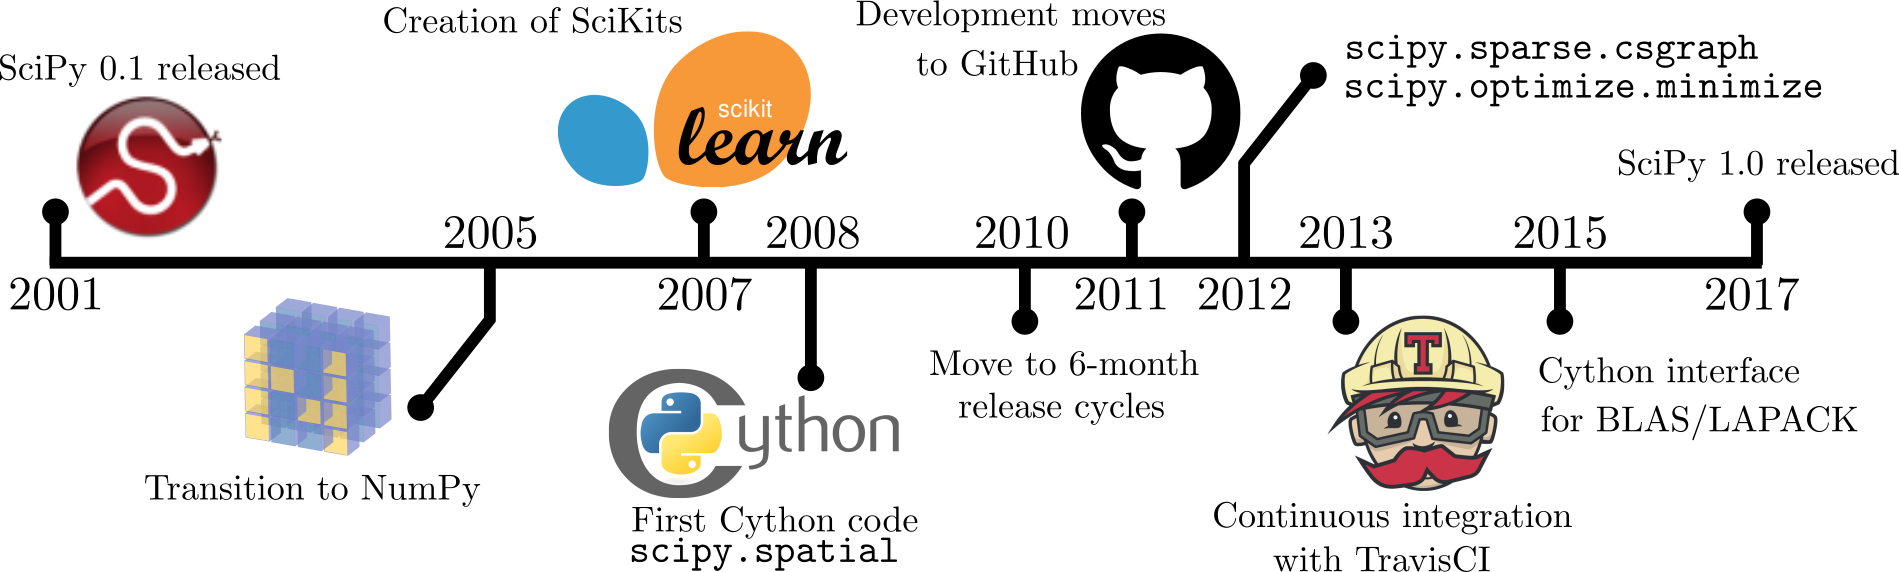
\includegraphics[width=0.95\textwidth]{static/scipy_timeline}
\caption{Major milestones from SciPy's initial release in 2001 to
the release of SciPy 1.0 in 2017. Logos reprinted with permission.}
\label{fig:timeline}
\end{figure}

% Release management

% Jarrod
%https://mail.python.org/pipermail/scipy-dev/2007-August/007613.html
%Ralf
%https://mail.python.org/pipermail/numpy-discussion/2010-March/049057.html
%https://mail.python.org/pipermail/scipy-dev/2010-March/014034.html
%https://mail.python.org/pipermail/scipy-dev/2010-April/014091.html


\section*{Architecture and implementation choices}
\subsection*{Project scope}

SciPy provides fundamental algorithms for scientific computing. The
breadth of its scope was derived from the Guide to Available Mathematical
Software classification system (GAMS\cite{boisvert1991guide}). In areas
that move relatively slowly, e.g. linear algebra, SciPy aims to provide
complete coverage. In other areas it aims to provide fundamental building
blocks while interacting well with other packages specialized in that area.
For example, SciPy provides what one expects to find in a
statistics textbook (probability distributions, hypothesis tests, frequency
statistics, correlation functions, and more), while 
Statsmodels\cite{statsmodels2010} provides
more advanced statistical estimators and inference methods;
scikit-learn\cite{pedregosa2011scikit} covers machine learning; and
PyMC3\cite{10.7717/peerj-cs.55}, emcee\cite{2013PASP-emcee} and 
PyStan\cite{pystan-ref} cover Bayesian statistics and probabilistic modeling.
scikit-image\cite{vanderwalt2014scikit} provides image processing
capabilities beyond \texttt{scipy.ndimage}, sympy\cite{meurer2017sympy}
provides a Python interface for symbolic computation, and
NetworkX\cite{hagberg2008networkx} is a Python library for probing
graphs and networks in a more specialized way than SciPy components
like \texttt{sparse.csgraph} or \texttt{spatial}.

We use the following criteria to determine whether or not to include new
functionality in SciPy:
\begin{itemize}
    \item The algorithm is of relevance to multiple fields of science.
    \item The algorithm is demonstrably important.  For example, it is classic
    enough to be included in textbooks, or it is based on a peer-reviewed article
    which has a significant number of citations.
\end{itemize}

In terms of software systems and architecture, SciPy's scope matches NumPy's:
algorithms for in-memory computing on single machines, with support for a wide
range of data types and process architectures. Distributed computing and support
for graphics processing units (GPUs) is explicitly out of scope.

\subsection*{Package organization}
The SciPy library is organized as a collection of subpackages.  The 16
subpackages include mathematical building blocks (e.g. linear algebra, Fourier
transforms, special functions), data structures (e.g. sparse matrices, $k$-D trees),
algorithms (e.g. numerical optimization and integration, clustering, interpolation,
graph algorithms, computational geometry), and higher-level data analysis
functionality (e.g. signal and image processing, statistical methods).

Here we summarize the scope and capabilities of each subpackage.

\begin{description}[leftmargin=!, labelwidth=\widthof{\bfseries \texttt{interpolate}}]
\itemsep0em
\item[\texttt{cluster}]
    The \texttt{cluster} subpackage contains two modules:
    \texttt{cluster.vq} provides vector quantization and $k$-means algorithms,
    and \texttt{cluster.hierarchy} provides functions for hierarchical and
    agglomerative clustering.
\item[\texttt{constants}]
    Physical and mathematical constants, including the CODATA recommended
    values of the fundamental physical constants\cite{CODATA2014}.
\item[\texttt{fftpack}]
    Fast Fourier Transform routines.  In addition to the FFT itself, the subpackage
    includes functions for the discrete sine and cosine transforms and for
    pseudo-differential operators.
\item[\texttt{integrate}]
    The \texttt{integrate} subpackage provides tools for the numerical
    computation of single and multiple definite integrals and for the
    solution of ordinary differential equations, including initial value
    problems and two-point boundary value problems.
\item[\texttt{interpolate}]
    The \texttt{interpolate} subpackage contains spline functions and
    classes, one-dimensional and multi-dimensional (univariate and
    multivariate) interpolation classes, Lagrange and Taylor polynomial
    interpolators, and wrappers for FITPACK and DFITPACK functions.
\item[\texttt{io}]
    A collection of functions and classes for reading and writing MATLAB, IDL,
    Matrix Market, Fortran, NetCDF, Harwell-Boeing, WAV and ARFF data files. 
\item[\texttt{linalg}]
    Linear algebra functions, including:
    elementary functions of a matrix, such as the trace, determinant, norm and
    condition number;
    basic solver for $Ax = b$;
    specialized solvers for Toeplitz matrices, circulant matrices, triangular
    matrices and other structured matrices; least squares solver and
    pseudo-inverse calculations; eigenvalue and eigenvector calculations
    (basic and generalized); matrix decompositions, including Cholesky, Schur,
    Hessenberg, $LU$, $LDL^{\intercal}$, $QR$, $QZ$, singular value, and polar;
    and functions to create specialized matrices, such as diagonal, Toeplitz,
    Hankel, companion, Hilbert, and more.
\item[\texttt{ndimage}]
    This package contains various functions for multi-dimensional image
    processing, including convolution and assorted linear and nonlinear
    filters (Gaussian filter, median filter, Sobel filter, etc.);
    interpolation; region labeling and processing; and mathematical morphology
    functions.
\item[\texttt{misc}]
    A collection of functions that did not fit into the other subpackages.
    While this subpackage still exists in SciPy 1.0, effort is underway
    to deprecate or relocate the contents of this subpackage and eventually remove it.
\item[\texttt{odr}]
    Orthogonal distance regression, including Python wrappers for the Fortran
    library ODRPACK.
\item[\texttt{optimize}]
    The package includes the following, with additional details in the SI:
    simplex and interior-point linear programming solvers,
		implementations of many nonlinear minimization algorithms,  
		a routine for least-squares curve fitting, and 
		a collection of general nonlinear solvers for root-finding.
\item[\texttt{signal}]
    The \texttt{signal} subpackage focuses on signal processing and
    basic linear systems theory.  Functionality includes
    convolution and correlation; splines; filtering and filter design;
    continuous and discrete time linear systems; waveform generation;
    window functions; wavelet computations; peak finding; and spectral
    analysis.  
\item[\texttt{sparse}]
    This package includes implementations of several representations of
    sparse matrices.  It contains two modules, 
    \texttt{scipy.sparse.linalg} and \texttt{scipy.sparse.csgraph}.

    \texttt{scipy.sparse.linalg} provides a collection of linear algebra
    routines that work with sparse matrices, including linear equation
    solvers, eigenvalue decomposition, singular value decomposition
    and LU factorization.

    \texttt{scipy.sparse.csgraph} provides a collections of graph algorithms
    for which the graph is represented using a sparse matrix.  Algorithms
    include connected components, shortest path, minimum spanning tree
    and more.
\item[\texttt{spatial}]
    This subpackage provides spatial data structures and algorithms,
    including the $k$-d tree, Delaunay triangulation, convex hulls and Voronoi
    diagrams.  The subpackage \texttt{scipy.spatial.distance} provides
    a large collection of distance functions, along with functions for
    computing the distance between all pairs of vectors in a given collection
    of points or between all pairs from two collections of points.
\item[\texttt{special}]
    The name comes the class of functions traditionally known as \emph{special
    functions}, but over time, the subpackage has grown to include functions
    beyond the classical special functions.  A more appropriate characterization
    of this subpackage is simply \emph{useful functions}.
    It includes a large collection of the classical special functions
    such as Airy, Bessel, etc.; orthogonal families of polynomials;
    the Gamma function, and functions related to it;
    functions for computing the PDF, CDF and quantile function for several
    probability distributions;
    information theory functions;
    combinatorial functions \texttt{comb} and \texttt{factorial};
    and more.
\item[\texttt{stats}]
    The \texttt{stats} subpackage provides a large collection of continuous
    and discrete \emph{probability distributions}, each with methods to compute
    the PDF or PMF, CDF, moments and other statistics, generation of random
    variates, and more;
    \emph{statistical tests}, including Pearson's correlation, Spearman's rank-order
    correlations, Kendall's tau, chi-squared test and its generalization as the
    Cressie-Read power divergence, contingency table tests including Fisher's
    exact test and Mood's median test, and many more;
    and assorted \emph{transformations and statistics} of data.
\end{description}


\subsection*{Language choices}

Python, Cython, Fortran, C and C++ are the programming languages used to
implement scientific algorithms in the SciPy library. An analysis of our code
base using the \texttt{linguist} library\cite{linguistref} provides a 
detailed breakdown as \% composition by programming language in 
SciPy (Figure~\ref{fig:linguist}).

\begin{figure}[H]
    \centering
		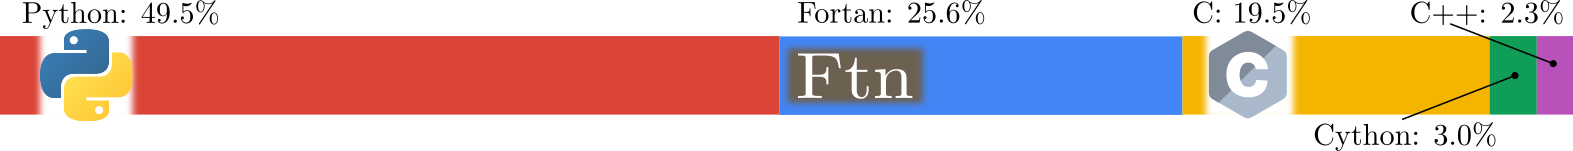
\includegraphics[width=\textwidth]{static/composition}
    \caption{The breakdown of programming languages used in the
             SciPy library determined using the linguist library.
    	 Small ($<0.5 \%$) amounts of TeX, Matlab, Shell,
    	 and Makefile are excluded for clarity and mostly
    	 provide supporting roles in tests, building, and
    	 documentation.}
    \label{fig:linguist}
\end{figure}

For implementing new functionality, we have a clear order of language
preference.  First Python, if performance is not an issue. If it is, then in
order of preference: Cython, C, C++, Fortran. The main motivation for this is
maintainability: Cython has the highest abstraction level and most Python
developers will understand it. C is also widely known, and easier to deal with
for the core development team than C++ and especially Fortran.

While it is not surprising that Python is heavily used in SciPy, the usage
distribution of the other languages warrants some discussion. Fortran is an
extremely well-established scientific programming language, both for historical
reasons and because of its continued excellent
performance\cite{Koelbel:1993:HPF:562354}. We wrap the FFTPACK Fortran library
for performing Fourier transforms\cite{SWARZTRAUBER198445, SWARZTRAUBER198251}
since this library has been a standard in the field for 33 years and has a
license that is compatible with our own. Likewise, we wrap the Fortran source
for ODEPACK\cite{citeulike:2644528} as it has been  trusted for the initial
value problem for ordinary differential equation systems for 30 years. For
similar reasons we also wrap the Fortran libraries
QUADPACK\cite{1983qspa.book.....P} (for numerical integration of
one-dimensional functions), FITPACK\cite{Dierckx:1993:CSF:151103}
(curve-fitting / interpolation), ODRPACK\cite{ODRPACK_Boggs} (orthogonal
distance regression), MINPACK\cite{osti_6997568} (minimization of linear and
nonlinear equations), ARPACK\cite{leh:sor:yan96} (solving large scale
eigenvalue problems), ALGORITHM 644\cite{Amos:1986:APP:7921.214331} (handling
Bessel Functions), and CDFLIB\cite{CDFLIB_site} (evaluation of cumulative
density functions).

Rounding out the top three languages in SciPy is C, which is also extremely
well-established over several decades\cite{Kernighan:1988:CPL:576122} of
scientific computing. Alongside its objected-oriented relative C++, C can be
leveraged in Python after being exposed using the Cython language. Cython has
been described as a creole language that mixes the best parts of Python and
lower-level C / C++ paradigms\cite{behnel2011cython}. We thus often use Cython
as a glue between well-established low-level scientific computing libraries and
the Python interface offered by SciPy. We also use Cython to enable performance
enhancements in Python code, especially for cases where heavily used inner
loops benefit from a compiled code with static typing. Some of the C libraries
that we wrap in SciPy include trlib\cite{doi:10.1080/10556788.2018.1449842}
(iterative solving of the trust region problem),
SuperLU\cite{li05,superlu_ug99} (solution of large, sparse, nonsymmetric
systems of linear equations), Qhull\cite{Barber:1996:QAC:235815.235821}
(computational geometry), and Cephes\cite{cephes_netlib} (mathematics
algorithms). 

Therefore, the relative abundance of different programming languages in the
SciPy library results from a combination of the usage of powerful performance
enhancing languages that interact well with Python (i.e., Cython), and the
usage of languages (and their libraries) that have proven reliable and
performant over many decades. The position that SciPy occupies near the
foundation of the scientific Python ecosystem is such that adoption of new
languages or major dependencies is generally unlikely---our choices are strongly
driven by long-term stability. GPU acceleration, new transpiling libraries, and
the latest JIT compilation approaches (i.e.,
Numba\cite{Lam:2015:NLP:2833157.2833162}) are very powerful, but currently fall
outside the remit of the main SciPy library. That said, we have recently
increased our efforts to support compatibility with some of these options, and
having our full test suite pass with the PyPy JIT
compiler\cite{Bolz:2009:TMP:1565824.1565827} is now a requirement in our
development workflow.

\subsection*{API and ABI evolution}

The application programming interface (API) for SciPy consists of approximately
1500 functions and classes.  Our policy for evolving the API over time is that
new functionality can be added, while removing or changing existing
functionality can only be done if the benefits of that exceeds the (often
significant) costs to users, \textit{and} only after giving clear deprecation
warnings to those users for at least one year. In general, we encourage
changes that improve clarity in the API of the library but strongly discourage
breaking backwards compatibility given our position near the base of the 
scientific Python computing stack.

In addition to the Python API, SciPy has C and Cython interfaces in a number
of submodules. Therefore, we have to also consider the application binary
interface (ABI). This ABI has been stable for a long time, and we aim to
evolve it only in a backwards compatible way.

\section*{Key technical improvements}
\label{sec:technical_improvements}
Here we describe key technical improvements made in the last three years.

\subsection*{Data structures}

\subsubsection*{Sparse matrices}

\texttt{scipy.sparse} offers seven sparse matrix data structures,
also known as sparse formats. The most important ones are the row- 
and column-compressed formats (CSR and CSC, respectively). 
These offer fast major-axis indexing and fast matrix-vector multiplication,
and are used heavily throughout SciPy and dependent packages.

Over the last three years our sparse matrix handling internals have been
rewritten and performance has been improved. Iterating over and slicing of CSC
and CSR matrices is now faster by up to 35\% (Figure~\ref{fig:sparse-iter}),
 and the COO / DIA to CSR / CSC matrix format
conversions are now faster (Figure~\ref{fig:sparse-conv}). Importantly,
SuperLU\cite{superlu_ug99} was updated to version 5.2.1, enhancing the
low-level implementations leveraged by a subset of our \texttt{sparse}
offerings.

From a new features standpoint, \texttt{scipy.sparse} matrices and linear
operators now support the Python matrix multiplication (@) operator when
available. We've added \texttt{scipy.sparse.norm} and
\texttt{scipy.sparse.random} for computing sparse matrix norms and drawing
random variates from arbitrary distributions, respectively. Also, we've made a
concerted effort to bring the \texttt{scipy.sparse} API into line with the
equivalent NumPy API where possible.

\subsubsection*{\texttt{cKDTree}}

The \texttt{cKDTree} module, which implements a space-partitioning data structure that
organizes points in $k$-dimensional space, was rewritten in C++ with templated classes. 
Support was added for periodic boundary conditions, which are often used 
in simulations of physical processes. 

In 2013, the time complexity of the $k$-nearest neighbor search from
\texttt{cKDTree.query} was approximately loglinear \cite{knn-jake},
consistent with its formal description \cite{kdtree-search-algo}.
Since then, we've enhanced \texttt{cKDTree.query} by reimplementing it in
C++, removing memory leaks, and allowing release of the global interpreter lock (GIL) so that
multiple threads may be used\cite{gh-4374}. This generally improved
performance on any given problem (Figure~\ref{fig:asvbench}) while
preserving the asymptotic complexity (Figure~\ref{fig:knn-complexity}).

In 2015, SciPy added the \texttt{sparse\_distance\_matrix} routine for generating 
approximate sparse distance matrices between \texttt{KDTree} objects by ignoring 
all distances that exceed a user-provided value. Also, this routine is not 
limited to the conventional L2 (Euclidean) norm but supports any Minkowski 
p-norm between 1 and infinity. By default, the returned data structure is a 
Dictionary Of Keys (DOK) based sparse matrix, which is very efficient for matrix 
construction. This hashing approach to sparse matrix assembly can be 7 times 
faster than constructing with CSR format
\cite{10.1007/978-3-540-75755-9_107}, and the C++ level sparse matrix construction 
releases the Python GIL for increased performance. Once the matrix is constructed, 
distance value retrieval has an amortized constant time complexity 
\cite{Cormen:2001:IA:580470}, and the DOK structure can be efficiently converted 
to a CSR, CSC, or COO matrix to allow for 
speedy arithmetic operations.

In 2015 the \texttt{cKDTree} dual tree counting algorithm\cite{Moore2000ar}
was enhanced to support weights\cite{ckdtree-weights}, which are
essential in many scientific applications, e.g. computing correlation
functions of galaxies\cite{0004-637X-750-1-38}.


\subsection*{Unified bindings to compiled code}

\subsubsection*{LowLevelCallable}

As of SciPy version 0.19, it is possible for users to wrap low-level functions
in a \texttt{scipy.LowLevelCallable()} object that reduces the overhead for
calling compiled C functions directly from Python.  Supported low-level
functions include \texttt{PyCapsule} objects, ctypes function pointers, and
cffi function pointers. The low level function signature must be consistent
with the expectations of the routine it is passed to. For example, the
documentation for \texttt{scipy.ndimage.generic\_filter} defines two acceptable
C callback function signatures that may be used to produce functions that
operate on each element of image data with low overhead. The C code may be
generated using numba or Cython, for example, as long as the function call
signature matches the specifications. Furthermore, it is even possible to
generate a low-level callback function automatically from a Cython module using
\texttt{scipy.LowLevelCallable.from\_cython}.

\subsection*{Cython bindings for BLAS, LAPACK, and special}

SciPy has provided special functions and leveraged BLAS and
LAPACK\cite{LAPACK} routines for many years. SciPy now additionally
includes Cython\cite{behnel2011cython} wrappers for:
many BLAS and LAPACK routines (added in 2015), and the special functions 
provided in the \texttt{scipy.{\allowbreak}special} submodule (added in 2016).  
These Cython wrappers are available in the modules
\texttt{scipy.{\allowbreak}linalg.{\allowbreak}cython\_blas},
\texttt{scipy.{\allowbreak}linalg.{\allowbreak}cython\_lapack}, and
\texttt{scipy.{\allowbreak}special.{\allowbreak}cython\_special} respectively.
When writing algorithms in Cython, it is typically more efficient to call
directly into the libraries SciPy wraps rather than indirectly, using SciPy's
Python APIs.  These low-level interfaces for Cython can also be used outside of
the SciPy codebase to gain access to the functions in the wrapped libraries
while avoiding the overhead of Python function calls.  This can give
performance gains of one or two orders of magnitude for many use cases.

Developers can also use the low-level Cython interfaces without linking against
the wrapped libraries\cite{blas-lapack-wrappers-scipy-2015}.  This lets other
extensions avoid the complexity of finding and using the correct libraries.
Avoiding this complexity is especially important when wrapping libraries
written in Fortran.  Not only can these low-level wrappers be used without a
Fortran compiler, they can also be used without having to handle all the
different Fortran compiler ABI's and name mangling schemes.

Most of these low-level Cython wrappers are generated automatically to help
with both correctness and ease of maintenance.  The wrappers for BLAS and
LAPACK are primarily generated using type information that is parsed from the
BLAS and LAPACK source files using F2PY\cite{peterson2009f2py}, though a small
number of routines use hand-written type signatures instead.  The input and
output types of each routine are saved in a data file that is read at build
time and used to generate the corresponding Cython wrapper files.  The wrappers
in \texttt{scipy.{\allowbreak}special.{\allowbreak}cython\_special} are also
generated from a data file containing type information for the wrapped
routines.

Since SciPy can be built with LAPACK 3.4.0 or later, Cython wrappers are only
provided for the routines that maintain a consistent interface across all
supported LAPACK versions.  The standard BLAS interface provided by the various
existing BLAS libraries is not currently changing, so changes are not generally
needed in the wrappers provided by SciPy.  Changes to the Cython wrappers for
the functions in \texttt{scipy.{\allowbreak}special} follow corresponding
changes to the interface of that submodule.

\subsection*{Numerical optimization}

\newcommand{\RR}{\ensuremath{\mathbb{R}}}
The \texttt{scipy.optimize} module provides functions for the numerical solution of several classes of root finding and optimization problems:
\begin{enumerate}
\item nonlinear root finding problems (\texttt{brentq}, \texttt{brenth}, \texttt{ridder}, \texttt{bisect}, \texttt{newton}, and \texttt{root}),
\item linear sum assignment problems (\texttt{linear\textunderscore sum\textunderscore assignment}),
\item linear and nonlinear sum-of-squares problems (\texttt{leastsq}, \texttt{least\textunderscore squares}, \texttt{nnls}, \texttt{lsq\textunderscore linear}, and \texttt{curve\textunderscore fit}),
\item general, linear optimization problems (\texttt{linprog}),
\item general, nonlinear, local optimization problems of a single variable (\texttt{minimize\textunderscore scalar}),
\item general, nonlinear, local optimization problems of several variables (\texttt{minimize}), and
\item general, nonlinear, global optimization problems of several variables (\texttt{basinhopping}, \texttt{brute}, \texttt{differential\textunderscore evolution}).
\end{enumerate}
Documentation of SciPy's functionality in each these areas can be found in (cite SciPy documentation), but here we highlight recent additions through SciPy 1.0.

%\subsubsection{Root Finding}
%The general ``root finding'' problem is to find a root $\mathbf{x} \in \RR^m$ of $\mathbf{f}: \RR^m \rightarrow \RR^m$, that is, to solve
%\begin{equation}
%\mathbf{f}(\mathbf{x}) = \mathbf{0}
%\end{equation}
%for a solution $\mathbf{x}$.\footnote{Equivalently the problem is to simultaneously find the roots $x_i \in \RR$ of several scalar functions $f_i : \RR \rightarrow \RR$, that is, to solve $f_i(x_0, x_1, \dots, x_{m-1}) = 0$ for $x_i$, $i \in \{0, 1, \dots {m-1}\}$.} The function \texttt{scipy.optimize.root} provides a common interface to several algorithms for solving problems of this type. For the special case\footnote{that is, to solve a single scalar equation $f(x) = 0$ for a single scalar variable $x$} $m = 1$, any one of several specialized functions \texttt{brentq}, \texttt{brenth}, \texttt{ridder}, \texttt{bisect}, or \texttt{newton} may provide improved performance or accuracy. (Have there been any recent improvements? Do we want to summarize the methods as @antonior92 has done for $minimize$? Do we have to explain that these methods only provide \emph{one} solution, and that they are iterative based on a user-provided guess? Do we have to explain the notion of tolerance? Is this a good template for the beginning of the following subsections?)


\subsubsection*{Linear Optimization}

A new interior-point optimizer for continuous linear programming problems, \texttt{linprog} with \texttt{method='interior-point'}, was released with SciPy 1.0. Implementing the core algorithm of the commercial solver MOSEK \cite{andersen2000mosek}, it solves all of the 90+ NETLIB LP benchmark problems \cite{netlib} tested. Unlike some interior point methods, this homogenous self-dual formulation provides certificates of infeasibility or unboundedness as appropriate. 

A presolve routine \cite{andersen1995presolving} solves trivial problems and otherwise performs problem simplifications, such as bound tightening and removal of fixed variables, and one of several routines for eliminating redundant equality constraints is automatically chosen to reduce the chance of numerical difficulties caused by singular matrices. Although the main solver implementation is pure Python, end-to-end sparse matrix support and heavy use of SciPy's compiled linear system solvers --- often for the same system with multiple right hand sides due to the predictor-corrector approach --- provide speed sufficient for problems with tens of thousands of variables and constraints.

Compared to the previously implemented simplex method, the new interior-point method is faster for all but the smallest problems, and is suitable for solving medium- and large-sized problems on which the existing simplex implementation fails. However, the interior point method typically returns a solution near the center of an optimal face, yet basic solutions are often preferred for sensitivity analysis and for use in mixed integer programming algorithms. This motivates the need for a crossover routine or a new implementation of the simplex method for sparse problems in a future release, either of which would require an improved sparse linear system solver with efficient support for rank-one updates

\subsubsection*{Nonlinear Optimization}


The \texttt{minimize} function provides methods for solving nonlinear optimization
problems. It unifies several methods with a common interface in order to facilitate
interchanging between solvers with different characteristics, summarized in Table~\ref{tab:minimize}.
%% Currently, this introduces a ton of whitespace around a very simple expression (min f(x)). The reader can easily find the standard of meaning of `nonlinear programming', so I believe it should be removed. If we decide that it is appropriate to include, then we should add the entire problem statement - including constraints - and we should also include the entire linear programming problem statement in the previous section.
% summarizes all the methods available for solving minimization problems of the type:
%\begin{equation}
%  \label{eq:minimization-prob}
%  \min_x f(x)
%\end{equation}
%where $f$ is a multivariate function $f: \mathbb{R}^n \rightarrow \mathbb{R}$ and $x \in \mathbb{R}^n$.
%%  Without the problem statement this sentence isn't really appropriate.
%\texttt{COBYLA} and \texttt{SLSQP} methods support nonlinear constraints, \texttt{L-BFGS-B} and \texttt{TNC} allow box constraints $x^l \le x \le x^u$,
%and the remaining methods are for unconstrained problems.

% The available methods implement a variety of solution strategies.
Derivative-free methods (e.g. \texttt{Nelder-Mead}, \texttt{Powell} and \texttt{COBYLA}) are appropriate for minimizing non-differentiable or
noisy objective functions. When derivatives are available, however, other methods offer faster convergence rates
and have proven convergence properties. 
The derivative-based methods start with an initial guess and refine it iteratively, seeking
a local solution to the optimization problem. Each of these algorithms implements one of two complementary strategies:
line-search or trust-region. At each iteration, the line-search (LS) methods choose a direction
and approximate the optimal point in the given direction. Trust-region (TR) methods, on the other
hand, choose a ``trust-region'' region for which a local model is valid and approximate the best point
inside.

One recently-added trust-region method is \texttt{trust-exact},
which achieves fast convergence by solving the trust-region subproblem almost exactly.
Unfortunately, it requires the Hessian to be stored and factored every iteration, which may preclude
the solution of large problems (e.g.~problems with more than 1000 variables).
Other methods are appropriate for large-scale problems, including
\texttt{CG}, which does not use second derivatives and thus has low memory requirements, and \texttt{L-BFGS-B}, which maintains a simple and compact representation of the Hessian.
\texttt{Newton-CG}, \texttt{trust-ncg} and \texttt{trust-krylov} use second order derivatives to achieve faster
convergence, but are still appropriate for large problems because they factorize the Hessian in an inexact and iterative way that does not require the Hessian to be stored.
The method \texttt{trust-krylov}, introduced in the latest release, is a good compromise between
\texttt{trust-ncg} and \texttt{trust-exact}: it provides a more accurate solution to the trust-region
subproblem than \texttt{trust-ncg}, but it does not require the Hessian to be stored and factored as in \texttt{trust-exact}.

While most \texttt{minimize} development prior to SciPy 1.0 has focused on unconstrained minimization, methods \texttt{SLSQP} and \texttt{COBYLA}\footnote{We note that any equality constraint $c_{\text{eq}}(x) = 0$ can be expressed as two inequality constraints $c_{\text{eq}}(x) \leq 0$ and $-c_{\text{eq}}(x) \leq 0$} support fully general nonlinear programming. However, neither provides special treatment for sparsity. Accordingly, ongoing development efforts for \texttt{minimize} are focused on the addition of nonlinear programming algorithms for large, sparse problems. 

\begin{table}[H]
  \centering
  \caption{Optimization methods from \texttt{minimize}, which solves problems of the form $\min_x f(x)$, where $x \in \mathbb{R}^n$ and $f: \mathbb{R}^n \rightarrow \mathbb{R}$ .  The field \textit{version added} specifies the algorithm's first appearance in SciPy. Algorithms with \textit{version added} ``0.6*'' were added in version 0.6 or before.
    The field \textit{wrapper} indicates whether the implementation available in SciPy wraps a function written in a compiled language
    (e.g. C or FORTRAN). The fields \textit{\nth{1}} and \textit{\nth{2} derivatives}
    indicates whether first or second order derivatives are required. When \textit{\nth{2} derivatives} is flagged
    with $\sim$ the algorithm does not requires second-order derivatives from
    the user; it computes an approximation internally and uses it to accelerate method convergence.
    \textit{Iterative Hessian factorization} denotes algorithms that factorize the Hessian in an iterative way,
    which does not require explicit matrix factorization or storage of the Hessian.
    \textit{Local convergence} gives a lower bound on the rate of convergence of the iterations sequence once the
    iterate is sufficiently close to the solution: linear (L), superlinear (S) and quadratic (Q). Convergence rates denoted S$^*$ indicate that the algorithm
    has a superlinear rate for the parameters used in SciPy, but can  achieve a quadratic convergence rate with other parameter choices.
    \textit{Global convergence} is marked for the algorithms with guarantees of convergence to a stationary
    point (i.e. a point $x^*$ for which $\nabla f(x^*) = 0$). The table also indicates which algorithms
    can deal with constraints on the variables. We distinguish between: \textit{bound constraints} (i.e. $x^l \le x \le x^u$),
    \textit{equality constraints} (i.e. $c_{\text{eq}}(x) = 0$) and \textit{inequality constraints} (i.e. $c_{\text{ineq}}(x) \ge 0$).}
  \begin{tabular}{cccccccccccccc}
      & \rotatebox{80}{\texttt{Nelder-Mead}} & \rotatebox{80}{\texttt{Powell}} & \rotatebox{80}{\texttt{COBYLA}} & \rotatebox{80}{\texttt{CG}} & \rotatebox{80}{\texttt{BFGS}}&  \rotatebox{80}{\texttt{L-BFGS-B}} & \rotatebox{80}{\texttt{SLSQP}} & \rotatebox{80}{\texttt{TNC}} & \rotatebox{80}{\texttt{Newton-CG}} & \rotatebox{80}{\texttt{dogleg}} & \rotatebox{80}{\texttt{trust-ncg}} & \rotatebox{80}{\texttt{trust-exact}} & \rotatebox{80}{\texttt{trust-krylov}} \\
    \hline
    Version added &  0.6* &  0.6* &  0.6* &  0.6* &  0.6* &  0.6* &  0.9 &  0.6* &  0.6* & 0.13 & 0.13 & 0.19 & 1.0 \\
    \hline
    Wrapper & & & \cmark & & & \cmark & \cmark & \cmark & &  & & & \cmark \\
    \hline
    \nth{1} derivatives &  & & & \cmark  & \cmark & \cmark & \cmark & \cmark & \cmark & \cmark & \cmark & \cmark & \cmark \\
    \hline
    \nth{2} derivatives &  &  &  &  & $\sim$ & $\sim$ & $\sim$ & \cmark & \cmark & \cmark & \cmark & \cmark & \cmark \\
    \hline
    \makecell{Iterative Hessian \\
    factorization} & & & &  & & & & \cmark & \cmark &  & \cmark &  & \cmark \\
    \hline
    Local convergence& & & & L & S &  L & S & S$^*$ & S$^*$ & Q & S$^*$ & Q & S$^*$  \\
    \hline
    Global convergence & & &  &   & \cmark & \cmark & \cmark & \cmark & \cmark & \cmark & \cmark & \cmark & \cmark  \\
    \hline
    \makecell{Line-search (LS) or\\ trust-region (TR)} & Neither  & LS &  TR & LS & LS & LS & LS & LS & LS & TR & TR & TR & TR \\
    \hline
    Bound constraints &&&\cmark&&&&\cmark&\cmark&\cmark&&&& \\
    \hline
    Equality constraints &&&&&&&\cmark&&&&& \\
    \hline
    Inequality constraint &&&\cmark&&&&\cmark&&&&& \\
    \hline
    References & \cite{nelder_simplex_1965, wright_direct_1996} & \cite{powell_efficient_1964} &
      \cite{powell_direct_1994, powell_direct_1998, powell_view_2007} &
      \cite{polak_note_1969, nocedal_numerical_2006} & \cite{nocedal_numerical_2006} & \cite{byrd_limited_1995, zhu_algorithm_1997} &
      \cite{schittkowski_nonlinear_1982, schittkowski_nonlinear_1982-1, schittkowski_convergence_1983, kraft_software_1988} &
      \cite{nash_newton-type_1984} & \cite{nocedal_numerical_2006}  & 
      \cite{powell_new_1970, nocedal_numerical_2006} &  \cite{steihaug_conjugate_1983, nocedal_numerical_2006} &
      \cite{conn_trust_2000, more_computing_1983} & \cite{gould_solving_1999, lenders_trlib:_2016} \\
    \hline
  \end{tabular}
  \label{tab:minimize}
\end{table}

Some problems may require the use of global optimizers to find the minimum of the objective function over the set of all parameter values, especially if the objective function possesses many local minima that other solvers could get stuck in.
\texttt{Brute} performs a grid search over the entire parameter range, with the best grid point undergoing further polishing by another solver. However, this approach becomes increasingly inefficient as the problem dimensionality increases, or if the objective function has many extrema.
\texttt{Basinhopping} \cite{Wales1997} uses random perturbation of the parameter vector, with local minimization. The acceptance of the new coordinates is dictated by the Metropolis test typically used in Monte Carlo simulations.
\texttt{differential\textunderscore evolution} \cite{Wormington1999,Storn1997} is a stochastic solver that improves by gradual evolution of a population of candidate solutions. In each iteration trial candidates are generated by combination of candidates from the existing population; if the trial candidates represent an improvement then the population is updated. \texttt{differential\textunderscore evolution} does not require that the objective function be differentiable.
%  basinhopping may need differentiable objective for the local minimization.
The SciPy benchmark suite possesses a comprehensive range of global optimization problems (196), of varying difficulties, that can be used to evaluate the performance of a particular solver. This suite is used to decide whether new solvers have good enough performance to be added to the package.

\subsection*{Statistical distributions}

The \texttt{scipy.stats} module provides more than 100 probability
distributions and a framework to implement additional distributions. Given an
expression for a probability distribution function (pdf), the framework will
calculate moments, cumulative distribution function (cdf), differential
entropy, and more. Those properties are calculated based on generic code, e.g.,
numerical integration of the pdf to obtain the cdf.  Where possible, the
generic code is replaced by explicit formulas or more accurate or efficient
implementations. For example, most distributions have an explicit formula for
the cdf, so it is used instead of integrating the pdf. The distributions
framework also allows the user to draw random variates from the distribution.
Drawing random variates now accepts a \texttt{random\_state} parameter, which
is either a \texttt{numpy.random.RandomState} object or an integer used to
generate such an object, to provide fine-grained user-level control over the
random state of a workflow.  Currently about 80 continuous univariate
distributions, 12 discrete univariate distributions and 10 multivariate
distributions are implemented.  Key recent distributions added to
\texttt{scipy.stats} include the histogram-based distribution in
\texttt{scipy.stats.rv\_histogram} and the multinomial distribution in
\texttt{scipy.stats.multinomial} (used, for example, in natural language
processing\cite{Griffiths5228}). \texttt{multinomial} is the first and so far
the only multivariate discrete distribution available in SciPy.

\subsection*{Polynomial interpolators}

Traditionally, SciPy relied heavily on the venerable \texttt{FITPACK}
Fortran library by P.~Dierckx \cite{Dierckx:1993:CSF:151103, FITPACK} for
univariate interpolation and approximation of data. The original monolithic
design and API for interaction between SciPy and FITPACK was limiting for both
users and developers, as detailed in the Supporting Information.

Implementing a new, modular design of polynomial interpolators was spread over
several releases. The goals of this effort were to have a set of basic objects
representing piecewise polynomials, to implement a collection of algorithms
for constructing various interpolators, and to provide users with building
blocks for constructing additional interpolators.

At the lowest level of the new design are classes which represent univariate
piecewise polynomials: \code{PPoly} (SciPy 0.13)\cite{scipy-gh2885},
\code{BPoly} (SciPy 0.13) and \code{BSpline} (SciPy 0.19)\cite{scipy-gh3174},
which allow
efficient vectorized evaluations, differentiation, integration and root-finding.
\code{PPoly} represents piecewise polynomials in the power basis in terms of
breakpoints and coefficients at each interval. \code{BPoly} is similar, and
represents piecewise polynomials in the Bernstein basis (which is suitable
for e.g., constructing Bezier curves). \code{BSpline} represents spline
curves, i.e., linear combinations of b-spline basis elements.\cite{deBoor1978} 

In the next layer, these polynomial classes are used for constructing several
common ways of interpolating data: \code{CubicSpline} (SciPy 0.18)
\cite{scipy-gh5653} constructs a twice 
differentiable piecewise cubic function, \code{Akima1DInterpolator} 
and \code{PCHIPInterpolator} implement two classic prescriptions for
constructing a $C^1$ continuous monotone shape-preserving interpolator.
\cite{FritschCarlson1980, Akima1970}


\subsection*{Test and benchmark suite}

\subsubsection*{Benchmark suite}

The airspeed velocity (asv\cite{asvref}) library enables benchmarking Python packages
over their lifetimes, and the performance of the SciPy code base was monitored
with asv starting in February of 2015 (PR \#4501). In addition to ensuring that
unit tests are passing (see Test suite section below), confirming 
that performance generally
remains constant or improves over the commit hash history of the project allows
us to objectively measure that our code base is improving, to empower
scientific applications.

Consider the asv benchmark results shown in Figure~\ref{fig:asvbench}, spanning
roughly nine years of project history. These demonstrate the gradual
performance improvements in a nearest-neighbor search through
\texttt{scipy.spatial.cKDTree.query()}, and can be run using:

\texttt{python run.py run -e -s 800 --bench "\textbackslash
btime\_query\textbackslash b" "02de46a546..b3ddb2c"},

where \texttt{run.py} is a light wrapper script around \texttt{asv}
that is packaged with SciPy.

\begin{figure}[H]
\centering
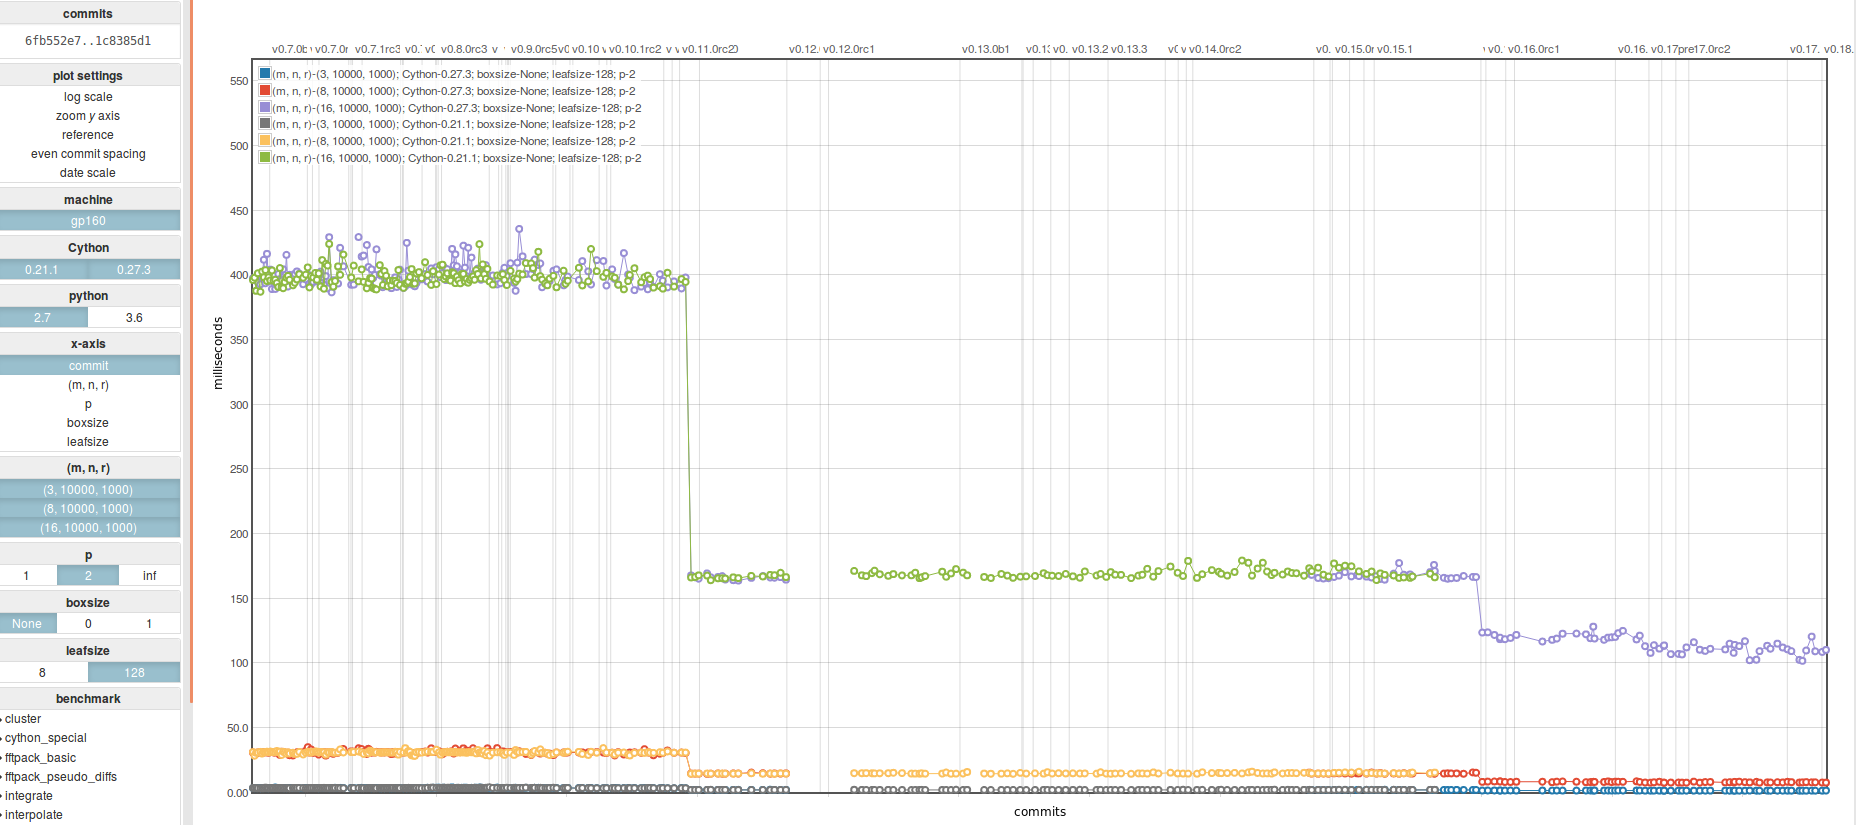
\includegraphics[width=\textwidth]{static/asv_time_query_ckdtree}
\caption{Airspeed velocity benchmarks for \texttt{scipy.spatial.cKDTree.query()}
over a roughly nine year commit history time frame. The results are based on
Python 2.7 performance on the master branch of the project using NumPy 1.8.2
and Cython versions 0.27.3, 0.21.1, and 0.18 (for improved backward
compatibility). Only the L2 (Euclidean) norm is shown here, and to improve
backward compatibility and sampling of the benchmarks there was no application
of toroidal topology to the \texttt{KDTree} (boxsize argument was ignored).}
\label{fig:asvbench}
\end{figure}

Any pull request can be compared against the \texttt{master} branch with the
command \texttt{asv continuous master new-feature}. This will provide a
benchmark against the master branch and the branch a new feature is implemented
in. More features are available in the \texttt{asv} documentation\cite{asvdocs}, including 
arguments to select which benchmarks to run.

\subsubsection*{Test suite}

The SciPy test suite is orchestrated by a continuous integration matrix that
includes POSIX and Windows (32/64-bit) platforms managed by Travis CI and
AppVeyor, respectively. Our tests cover Python versions 2.7, 3.4, 3.5, 3.6, and
include code linting with \texttt{pyflakes} and \texttt{pycodestyle}. There are more than $13,000$
unit tests in the test suite, which is written for usage with the \texttt{pytest}
framework, and with 87 \% and 45 \% line coverages for Python and compiled
code, respectively at the SciPy 1.0 release point (Figure~\ref{fig:coverage}). Documentation for the code is automatically built and hosted by
the CircleCI service to facilitate evaluation of documentation changes /
integrity.  Our full test suite also passes with PyPy3, a just-in-time compiled
version of the Python language.

\begin{figure}[H]
\centering
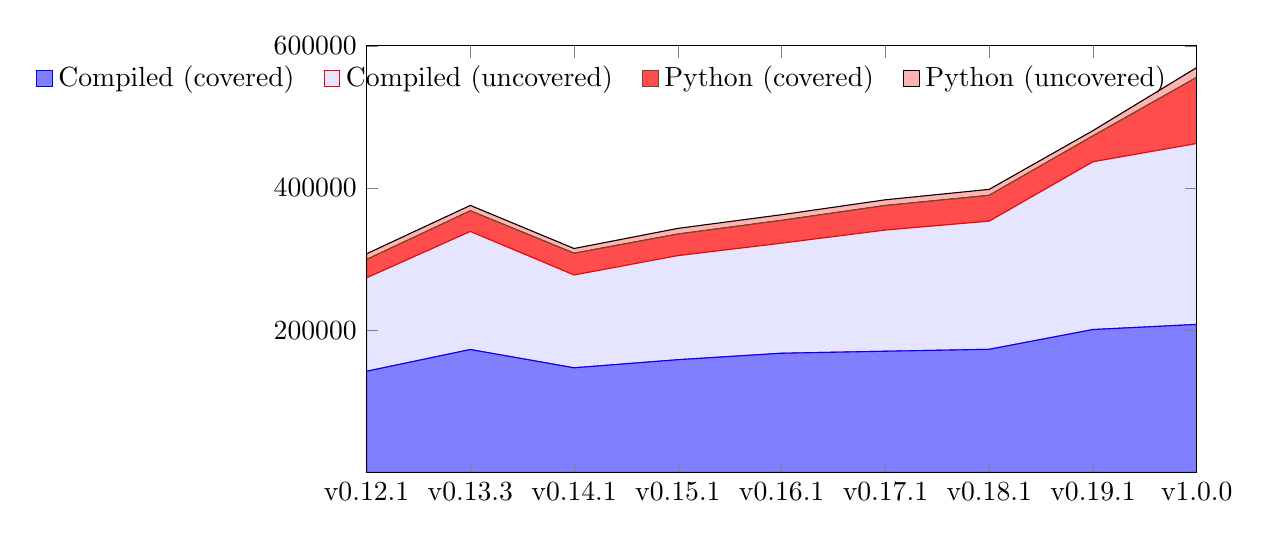
\begin{tikzpicture}[]
\pgfplotstableread[column/ver/.style=string type]{
ver totpyline covpyline uncovpyline totcompline covcompline uncovcompline
v0.12.1 33844 25721 8123 273634  142290 131344
v0.13.3 36638 28944 7694 338926  172852 166074
v0.14.1 37301 30587 6714 277643  147151 130492
v0.15.1 38339 30288 8051 304898  158547 146351
v0.16.1 40094 32075 8019 322398  167647 154751
v0.17.1 42566 34478 8088 340903  170452 170451
v0.18.1 44711 36216 8495 353417  173174 180243
v0.19.1 43823 36373 7450 436900  200974 235926
v1.0.0 106878 92984 13894 462574 208158 254416
}\covtable
    \begin{axis}[
    width=\textwidth,
    height=7cm,
    enlargelimits=false,
    ymin=0,
    ymax=6e5,
    stack plots=y,%   
    area style,
    xtick=data,
    ytick={2e5,4e5,6e5},
    xticklabels from table={\covtable}{ver},
    scaled y ticks=false,
    y tick label style={/pgf/number format/.cd, fixed, 1000 sep={}},
    legend entries={Compiled (covered),Compiled (uncovered),Python (covered),Python (uncovered)},
    legend style={draw=none,fill=none, cells={align=left},/tikz/every even column/.append style={column sep=3mm}},
    legend columns=-1,
    legend image code/.code={\fill[#1] (0cm,-0.1cm) rectangle (0.2cm,0.1cm);},
    ]
  \addplot+[fill=blue!50] table[x expr=\coordindex, y=covcompline] {\covtable} \closedcycle;
  \addplot+[fill=blue!10] table[x expr=\coordindex, y=uncovcompline] {\covtable} \closedcycle;
  \addplot+[fill=red!70] table[x expr=\coordindex, y=covpyline] {\covtable} \closedcycle;
  \addplot+[fill=red!30] table[x expr=\coordindex, y=uncovpyline] {\covtable} \closedcycle;
\end{axis}
\end{tikzpicture}
\caption{
Python (red) and compiled (blue) code volume in SciPy over time.
Deep-shaded area represents lines of code covered by units tests;
light-shaded area represents lines not covered. With the exception
of the removal of $\approx 61,000$ lines of compiled code for SciPy
v0.14, the volume of both compiled and Python
code has increased between releases, as has the number of lines
covered by unit tests. SciPy v1.0.0 was composed of $462,574$ lines of
compiled code with test coverage near $45 \%$ and $106,878$ lines of 
Python code with test coverage near $87 \%$.\\
The reconstitution of historical
build and test environments was performed using a docker-based approach
\cite{scipy-cov}. Analysis of lines of source code covered is performed 
automatically in our continuous integration suite using the \texttt{pytest-cov}
and \texttt{gcov} libraries. Some decreases in compiled code coverage may reflect
inclusion of additional vendored code.}
\label{fig:coverage}
\end{figure}

% NOTE: is there a citation for PyPy?

\section*{Project organization and community}

\subsection*{Governance}

SciPy adopted an official Governance Document on August 3, 2017\cite{SciPyProjectGovernance}. A Steering Council, currently composed of 18 members, oversees daily development of the project by contributing code and reviewing contributions from the community. Council Members have commit rights to the project repository, but they are expected to merge changes only when there are no substantive community objections. The Chair of the Steering Council, Ralf Gommers, is responsible for initiating biannual technical reviews of project direction and summarizing any private Council activities to the broader community. The project's Benevolent Dictator for Life (BDFL), Pauli Virtanen, has overruling authority on any matter, but the BDFL is expected to act in good faith and only exercise this authority when the Steering Council cannot reach agreement.

SciPy's official Code of Conduct was approved on October 24, 2017. In summary, there are five Specific Guidelines:
\emph{be open} to everyone participating in our community;
\emph{be empathetic and patient} in resolving conflicts;
\emph{be collaborative}, as we depend on each other to build the library;
\emph{be inquisitive}, as early identification of issues can prevent serious consequences; and
\emph{be careful with wording}.
The Code of Conduct specifies how breaches can be reported to a Code of Conduct Committee, and outlines procedures for the Committee's response. Our Diversity Statement ``welcomes and encourages participation by everyone''.


\subsection*{Community beyond the SciPy library}

The scientific Python ecosystem includes many examples
of domain-specific software libraries building on top
of SciPy features, and then returning to the base SciPy library
to suggest and even implement improvements to enable
more effective science applications. For example, there
are common contributors to the SciPy and Astropy core
libraries\cite{astropy-2018}, and what works well for 
one of the codebases, infrastructures, or communities 
is often transferred in some form to the other. At the codebase 
level, the \texttt{binned\_statistic} functionality
is one such cross-project contribution---it was initially
developed in an Astropy-affiliated package
and then placed in SciPy afterwards.

\subsection*{Maintainers and contributors}

The SciPy project has approximately 15 active maintainers---people who review
others' contributions, and in general do everything needed to ensure that the
software and the project move forward. Maintainers are critical to the health
of the project\cite{eghbal2016}; their skills and efforts largely determine how
fast the project moves forward, and they enable contributions from a much
larger group. Accordingly, the project also has an additional ~100 unique
contributors for every 6-monthly release cycle. Anyone with the interest and
skills can become a contributor or maintainer; the SciPy Developer
Guide\cite{scipy-dev-guide} provides guidance on how to do that.

\section*{Discussion}

% The Discussion should be succinct and must not contain subheadings.

SciPy has a strong developer community and a massive user base. GitHub traffic
metrics report roughly 20,000 unique visitors to the source website between May
14 and May 27, 2018, with 721 unique copies (``clones") of the codebase over
that roughly two-week period. The developer community at that time consisted of 610 unique
contributors of source code, with $>19,000$ commits accepted into the codebase
(GitHub page data).

From the user side, there were 13,096,468 downloads of SciPy from the Python
Packaging Index (PyPI) during the year 2017\cite{pypinfo}, which is a lower
bound on the number of total downloads by users given that downloading from
PyPI is only one of several popular methods to install SciPy.  The SciPy
website\cite{SciPylib}, which has been the default citation in the absence of a
peer-reviewed paper, has been cited $>3000$ times. Some of the most prominent
usages of or demonstrations of credibility for SciPy include the LIGO / Virgo
scientific collaboration that lead to the observation of gravitational waves
\cite{PhysRevLett.116.061102}, the fact that SciPy is shipped directly with
MacOS and in the Intel Distribution for Python\cite{intel-python}, and that SciPy is used
by 47 \% of all machine learning projects on GitHub\cite{octoverse-scipy}.

The SciPy Roadmap\cite{SciPy_roadmap_1,SciPy_roadmap_dev} is a
continuously-updated document
maintained by the community that describes some of the major directions for
improvement for the project, as well as specific limitations and matters that
require assistance moving forward.

We are still striving to increase the number of SciPy usage tutorials beyond
our current 15 section offering\cite{SciPy_tutorials}, but our standard
documentation for library features is already in excellent shape.

The low-level Cython code in our library (which interacts with C-level code and
exposes it for Python usage) could use some measure of modernization, including
migration to typed memoryviews to handle NumPy arrays instead of the older
syntax:

\begin{lstlisting}[language=Python]
# example of a function that takes a single
# 3 dimensional typed memoryview as an argument
# this allows Cython-level handling of a NumPy
# array object
cpdef int func_new(int[:, :, :] arr):
    pass

# example of the old syntax for handling
# the same scenario
cpdef int func_old(object[int, ndim=3, mode='strided'] arr):
    pass
\end{lstlisting}

Some additional roadmap items are summarized in Table~\ref{table:roadmap}.

\begin{table}[H]
\caption{Summary of SciPy Roadmap items following 1.0 release}
\begin{tabular}{ c|c }
    SciPy submodule & Summary of Change \\
    \hline
    \texttt{optimize} & a few more high quality global optimizers\\
    \texttt{fftpack} & reduce overlap with NumPy equivalent \\
    \texttt{linalg} & reduce overlap with NumPy equivalent \\
    \texttt{interpolate} & new spline fitting and arithmetic routines \\
    \texttt{interpolate} & new transparent tensor-product splines\\
    \texttt{interpolate} & new Non-Uniform Rational B-Splines\\
    \texttt{interpolate} & mesh refinement \& coarsening of B-splines and tensor products\\
    \texttt{signal} & migrate spline functionality to \texttt{interpolate}\\
    \texttt{signal} & Second Order Sections update to match capabilities in other routines\\
    \texttt{linalg} & support a more recent version of LAPACK\\
    \texttt{ndimage} & clarify usage of the ``data point'' coordinate
    model, and add additional wrapping modes\\
    \texttt{sparse} & incorporate sparse arrays from Sparse package\cite{abbasi2018sparse} \\
    \texttt{sparse.linalg} & add PROPACK wrappers for faster SVD\\
    \texttt{spatial} & add support for (quaternion) rotation matrices\\
    \texttt{special} & precision improvements for hypergeometric, parabolic cylinder, and spheroidal wave functions\\
\end{tabular}\label{table:roadmap}
\end{table}

\bibliography{references}

\section*{Acknowledgments}

\fixme{TODO}

%Acknowledgements should be brief, and should not include thanks to anonymous
%referees and editors, or effusive comments. Grant or contribution numbers may
%be acknowledged.

\section*{Author contributions statement}

\fixme{TODO}

%Must include all authors, identified by initials, for example: A.A.
%conceived the experiment(s),  A.A. and B.A. conducted the experiment(s), C.A.
%and D.A. analysed the results.  All authors reviewed the manuscript.

\section*{Additional information}

\fixme{TODO}

\section*{Supporting Information}

% separate Figure / Table numbering for SI
\renewcommand{\thefigure}{S\arabic{figure}}
\renewcommand{\thetable}{S\arabic{table}}
\setcounter{figure}{0}
\setcounter{table}{0}

\begin{figure}[H]
\centering
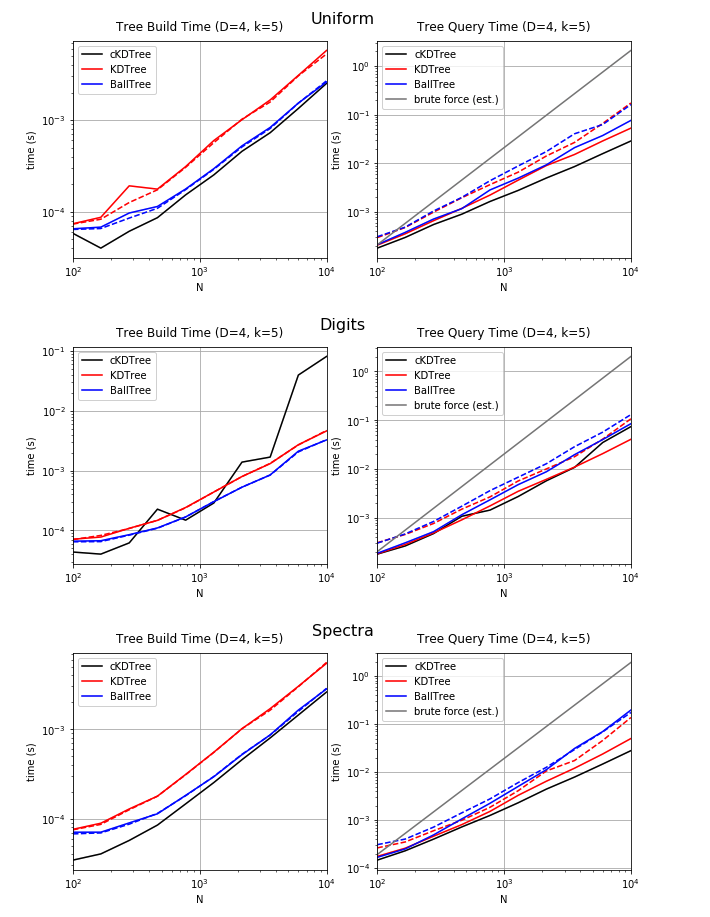
\includegraphics[width=0.8\textwidth]{supporting_info/knn_complexity_confirm}
\caption{Assessment of \texttt{cKDTree} nearest neighbor query time complexity as a function of the number of input points (N) along with similar assessment for related algorithms in scikit-learn. The calculations are based on code previously reported\cite{knn-jake}, but updated to use SciPy 1.0.0, Python 3.6, NumPy 1.13.1, and Cython 0.27.3.}
\label{fig:knn-complexity}
\end{figure}

\begin{figure}[H]
\centering
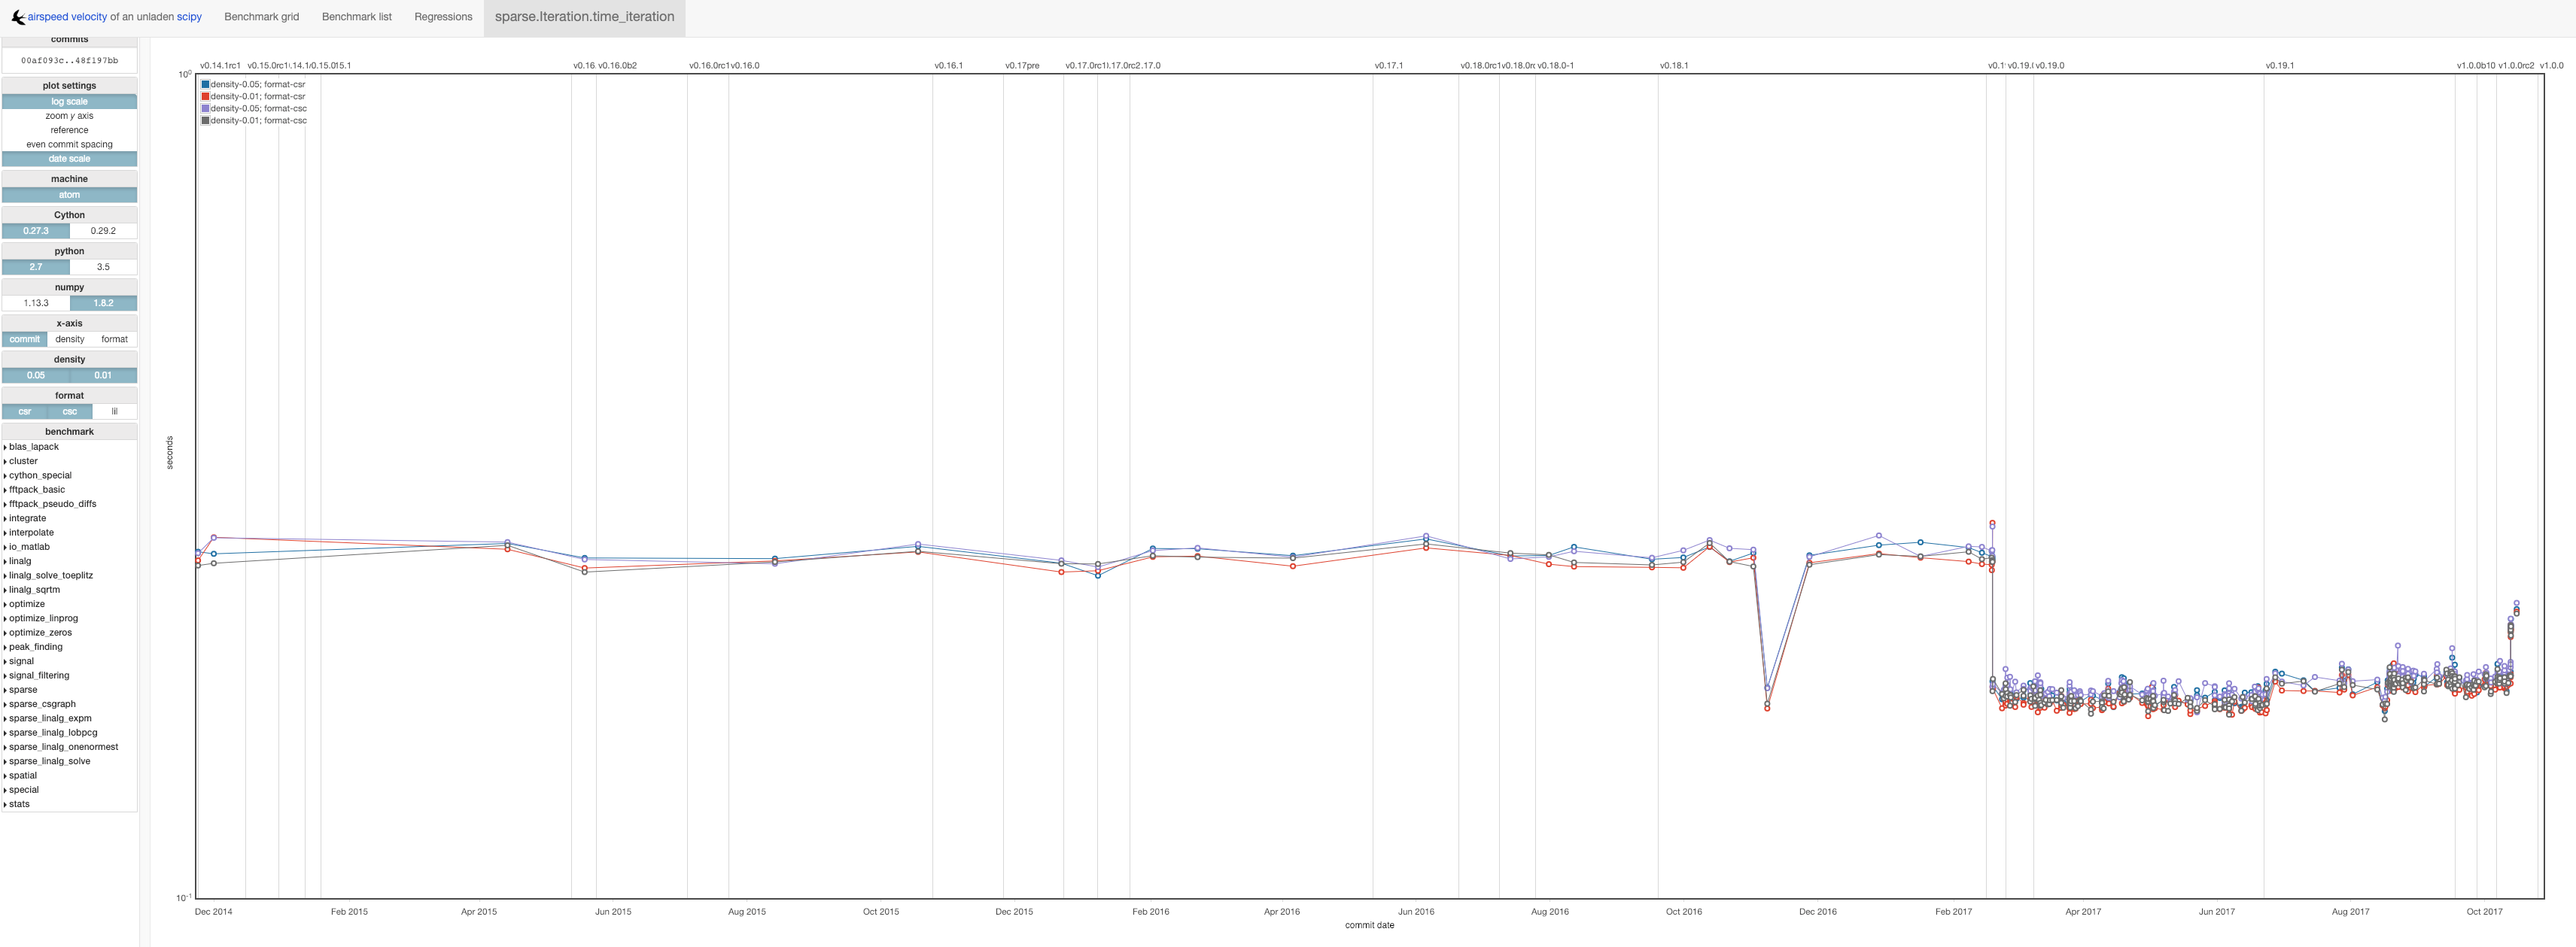
\includegraphics[width=\textwidth]{supporting_info/asv_bench/sparse/sparse_iteration_bench}
\caption{Airspeed velocity benchmarks for SciPy CSC and CSR matrix row iteration over roughly three years of commits prior to the release of version 1.0. Python version 2.7, Cython version 0.27.3, NumPy 1.8.2, and the indicated non-zero element density fractions were used. The partial performance regression observed shortly after the 1.0 release is likely related to a correctness fix\cite{sparse-regress}. The values were obtained from our regularly-updated suite of performance results available online at \url{http://pv.github.io/scipy-bench/}.}
\label{fig:sparse-iter}
\end{figure}

\begin{figure}[H]
\centering
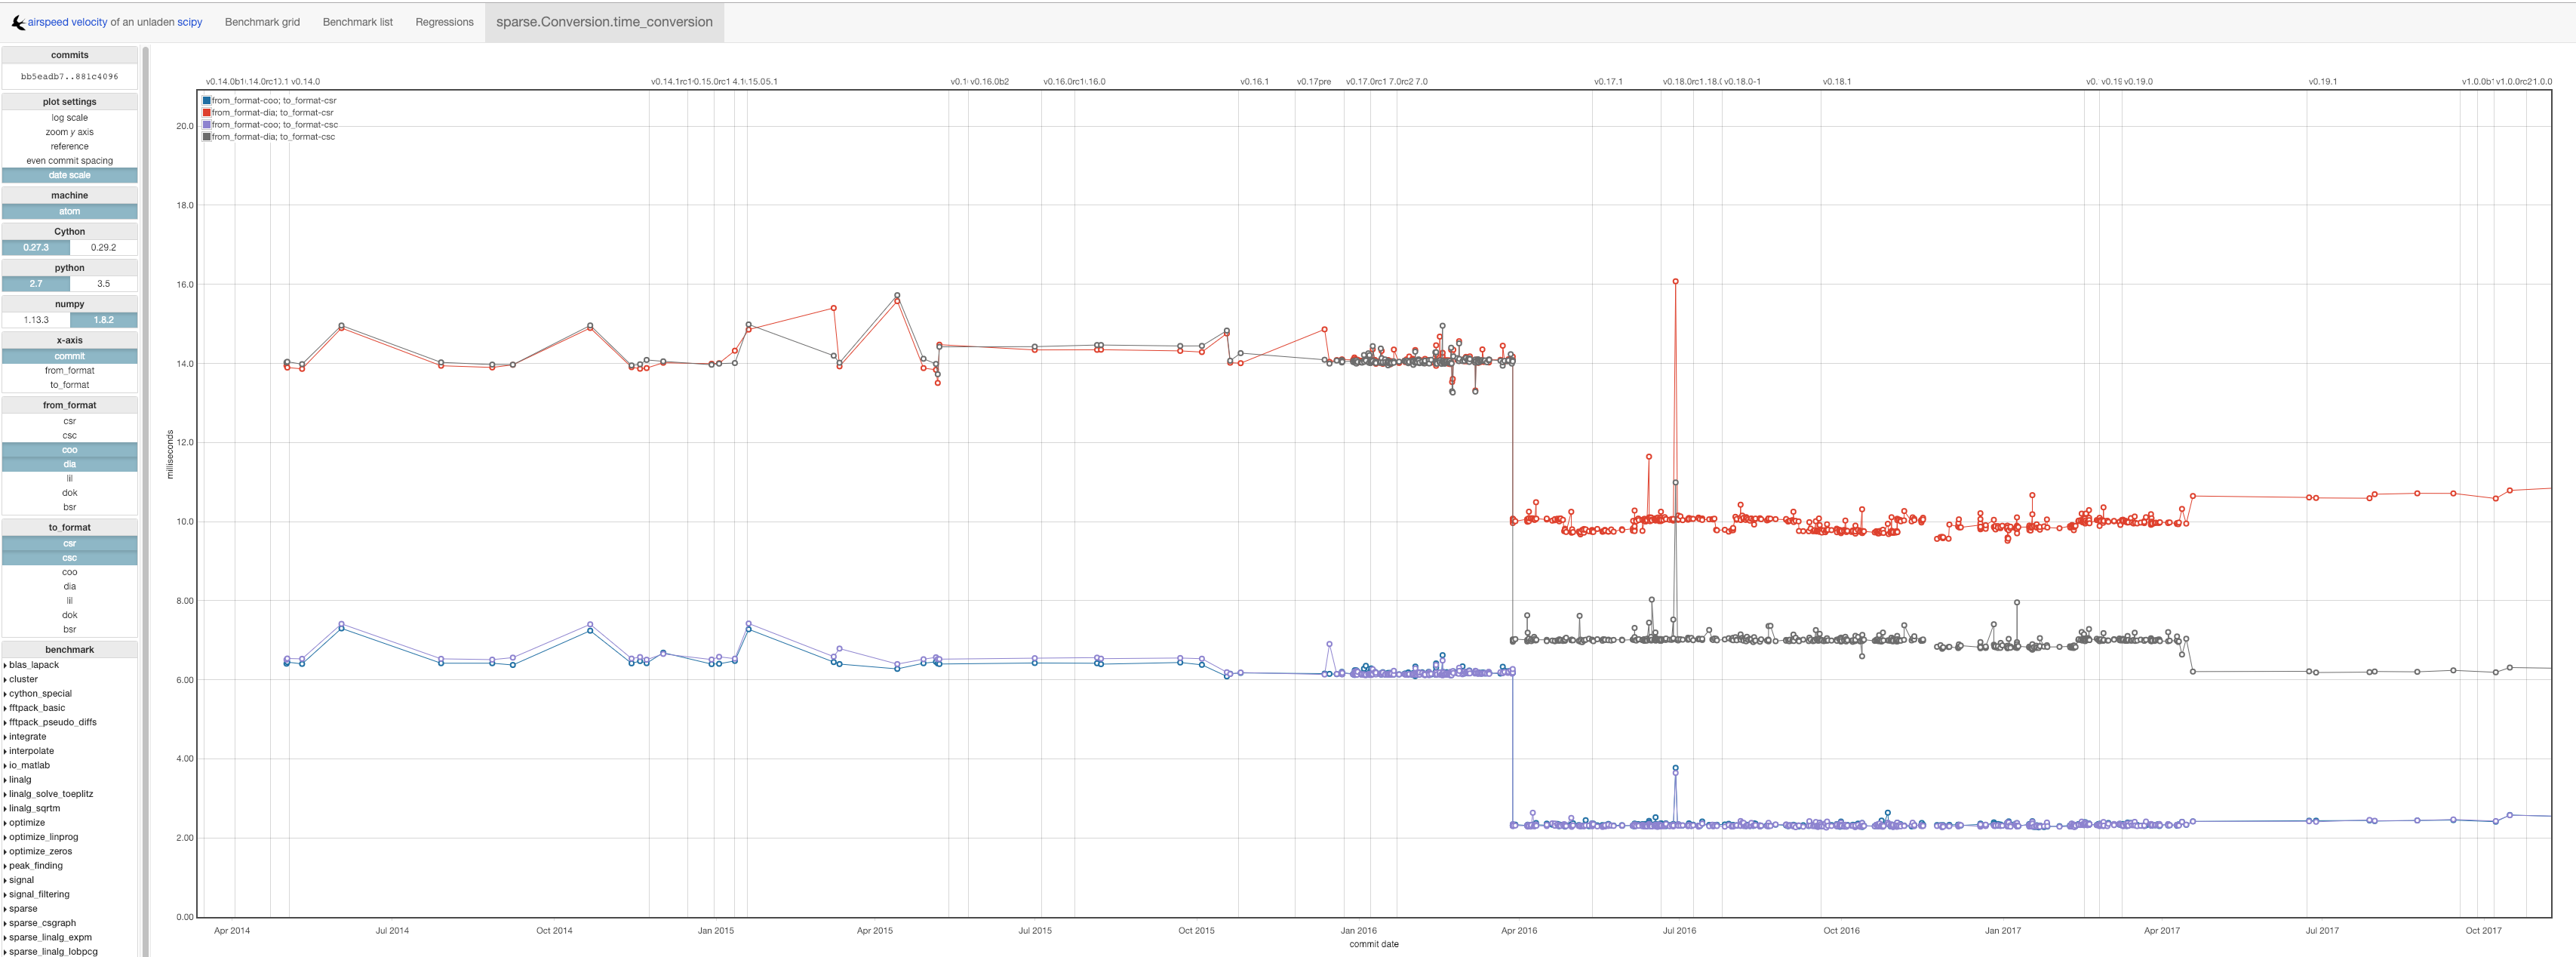
\includegraphics[width=\textwidth]{supporting_info/asv_bench/sparse/sparse_coo_dia_to_csr_csc}
\caption{Airspeed velocity benchmarks for SciPy COO / DIA to CSR / CSC matrix format conversion over roughly three years of commits prior to the release of version 1.0. Python version 2.7, Cython version 0.27.3, and NumPy 1.8.2 were used. The values were obtained from our regularly-updated suite of performance results available online at \url{http://pv.github.io/scipy-bench/}.}
\label{fig:sparse-conv}
\end{figure}

\section{Polynomial Interpolators: Additional Details}
FITPACK provides a collection of routines for calculating
smoothing splines and automatic knot selection. One issue 
with FITPACK and its Python wrappers in SciPy, \code{UnivariateSpline}
and the \code{splrep}/\code{splev} combination, is the monolithic design:
specific algorithms for construction of interpolating and 
smoothing splines and knot selection are tightly coupled 
at the Fortran level. The library offers a very
limited degree of user control over the details 
of the spline fitting it performs. 
%
Routines for manipulating piecewise polynomials and b-splines were either
not available or lacking in ease of use and/or performance characteristics.

An alternative set of spline interpolation routines was implemented in the
(now deprecated) \code{splmake}/\code{spleval} combination, and used as a
backend of the \code{interp1d} routine. To further complicate matters,
the spline format used by \code{splmake}/\code{spleval} was incompatible 
with \code{splrep}/\code{splev}.

Using \code{UnivariateSpline} in new code is not recommended. Given data points,
the helper function \code{make\_interp\_spline} constructs a \code{BSpline}
instance, representing a spline which interpolates the data. Interpolated values
at intermediate points can be computed either via its \code{\_\_call\_\_} method,
or by calling \code{splev(xnew, BSpline\_object)} --- the \code{splev} routine
accepts both \code{tck} tuples and \code{Bspline} instances.

Fitting \emph{smoothing} splines to data can currently only be done with 
FITPACK. Building alternative algorithms is certainly possible,
but is still to be implemented.

Interpolation with known or estimated derivatives, i.e., cubic or
higher-order Hermite splines, can be constructed by either
subclassing \code{PPoly} or \code{BPoly}, or using the factory
method \code{BPoly.from\_derivatives}.

The spline representation used by \code{BSpline} is directly
compatible with FITPACK. We recommend that users work with
\code{BSpline} objects instead of directly manipulating \code{tck}
tuples of knots, coefficients and the spline degree.

\section*{Numerical Optimization: Additional Details}
The \texttt{scipy.optimize} module provides functions for the numerical solution of several classes of root finding and optimization problems:
\begin{enumerate}
\item nonlinear root finding problems (\texttt{brentq}, \texttt{brenth}, \texttt{ridder}, \texttt{bisect}, \texttt{newton}, and \texttt{root}),
\item linear sum assignment problems (\texttt{linear\textunderscore sum\textunderscore assignment}),
\item linear and nonlinear sum-of-squares problems (\texttt{leastsq}, \texttt{least\textunderscore squares}, \texttt{nnls}, \texttt{lsq\textunderscore linear}, and \texttt{curve\textunderscore fit}),
\item general, linear optimization problems (\texttt{linprog}),
\item general, nonlinear, local optimization problems of a single variable (\texttt{minimize\textunderscore scalar}),
\item general, nonlinear, local optimization problems of several variables (\texttt{minimize}), and
\item general, nonlinear, global optimization problems of several variables (\texttt{basinhopping}, \texttt{brute}, \texttt{differential\textunderscore evolution}).
\end{enumerate}

\begin{table}[H]
  \centering
  \caption{Optimization methods from \texttt{minimize}, which solves problems of the form $\min_x f(x)$, where $x \in \mathbb{R}^n$ and $f: \mathbb{R}^n \rightarrow \mathbb{R}$ .  The field \textit{version added} specifies the algorithm's first appearance in SciPy. Algorithms with \textit{version added} ``0.6*'' were added in version 0.6 or before.
    The field \textit{wrapper} indicates whether the implementation available in SciPy wraps a function written in a compiled language
    (e.g. C or FORTRAN). The fields \textit{\nth{1}} and \textit{\nth{2} derivatives}
    indicates whether first or second order derivatives are required. When \textit{\nth{2} derivatives} is flagged
    with $\sim$ the algorithm does not requires second-order derivatives from
    the user; it computes an approximation internally and uses it to accelerate method convergence.
    \textit{Iterative Hessian factorization} denotes algorithms that factorize the Hessian in an iterative way,
    which does not require explicit matrix factorization or storage of the Hessian.
    \textit{Local convergence} gives a lower bound on the rate of convergence of the iterations sequence once the
    iterate is sufficiently close to the solution: linear (L), superlinear (S) and quadratic (Q). Convergence rates denoted S$^*$ indicate that the algorithm
    has a superlinear rate for the parameters used in SciPy, but can  achieve a quadratic convergence rate with other parameter choices.
    \textit{Global convergence} is marked for the algorithms with guarantees of convergence to a stationary
    point (i.e. a point $x^*$ for which $\nabla f(x^*) = 0$); this is \emph{not} a guarantee of convergence to a global minimum. The table also indicates which algorithms
    can deal with constraints on the variables. We distinguish among \textit{bound constraints} (i.e. $x^l \le x \le x^u$),
    \textit{equality constraints} (i.e. $c_{\text{eq}}(x) = 0$) and \textit{inequality constraints} (i.e. $c_{\text{ineq}}(x) \ge 0$).}
  \begin{tabular}{cccccccccccccc}
      & \rotatebox{80}{\texttt{Nelder-Mead}} & \rotatebox{80}{\texttt{Powell}} & \rotatebox{80}{\texttt{COBYLA}} & \rotatebox{80}{\texttt{CG}} & \rotatebox{80}{\texttt{BFGS}}&  \rotatebox{80}{\texttt{L-BFGS-B}} & \rotatebox{80}{\texttt{SLSQP}} & \rotatebox{80}{\texttt{TNC}} & \rotatebox{80}{\texttt{Newton-CG}} & \rotatebox{80}{\texttt{dogleg}} & \rotatebox{80}{\texttt{trust-ncg}} & \rotatebox{80}{\texttt{trust-exact}} & \rotatebox{80}{\texttt{trust-krylov}} \\
    \hline
    Version added &  0.6* &  0.6* &  0.6* &  0.6* &  0.6* &  0.6* &  0.9 &  0.6* &  0.6* & 0.13 & 0.13 & 0.19 & 1.0 \\
    \hline
    Wrapper & & & \cmark & & & \cmark & \cmark & \cmark & &  & & & \cmark \\
    \hline
    \nth{1} derivatives &  & & & \cmark  & \cmark & \cmark & \cmark & \cmark & \cmark & \cmark & \cmark & \cmark & \cmark \\
    \hline
    \nth{2} derivatives &  &  &  &  & $\sim$ & $\sim$ & $\sim$ & \cmark & \cmark & \cmark & \cmark & \cmark & \cmark \\
    \hline
    \makecell{Iterative Hessian \\
    factorization} & & & &  & & & & \cmark & \cmark &  & \cmark &  & \cmark \\
    \hline
    Local convergence& & & & L & S &  L & S & S$^*$ & S$^*$ & Q & S$^*$ & Q & S$^*$  \\
    \hline
    Global convergence & & &  &   & \cmark & \cmark & \cmark & \cmark & \cmark & \cmark & \cmark & \cmark & \cmark  \\
    \hline
    \makecell{Line-search (LS) or\\ trust-region (TR)} & Neither  & LS &  TR & LS & LS & LS & LS & LS & LS & TR & TR & TR & TR \\
    \hline
    Bound constraints &&&\cmark&&&&\cmark&\cmark&\cmark&&&& \\
    \hline
    Equality constraints &&&&&&&\cmark&&&&& \\
    \hline
    Inequality constraint &&&\cmark&&&&\cmark&&&&& \\
    \hline
    References & \cite{nelder_simplex_1965, wright_direct_1996} & \cite{powell_efficient_1964} &
      \cite{powell_direct_1994, powell_direct_1998, powell_view_2007} &
      \cite{polak_note_1969, nocedal_numerical_2006} & \cite{nocedal_numerical_2006} & \cite{byrd_limited_1995, zhu_algorithm_1997} &
      \cite{schittkowski_nonlinear_1982, schittkowski_nonlinear_1982-1, schittkowski_convergence_1983, kraft_software_1988} &
      \cite{nash_newton-type_1984} & \cite{nocedal_numerical_2006}  & 
      \cite{powell_new_1970, nocedal_numerical_2006} &  \cite{steihaug_conjugate_1983, nocedal_numerical_2006} &
      \cite{conn_trust_2000, more_computing_1983} & \cite{gould_solving_1999, lenders_trlib:_2016} \\
    \hline
  \end{tabular}
  \label{tab:minimize-si}
\end{table}

%To include, in this order: \textbf{Accession codes} (where applicable);
%\textbf{Competing financial interests} (mandatory statement).

%The corresponding author is responsible for submitting a
%\href{http://www.nature.com/srep/policies/index.html#competing}{competing
%financial interests statement} on behalf of all authors of the paper. This
%statement must be included in the submitted article file.

\end{document}

%%% Local Variables:
%%% mode: latex
%%% TeX-master: t
%%% End:
